\subsection{Estudo de Caso Emp\'irico}\label{subsec:estudo-de-caso-base}


A previsão da demanda de água é uma preocupação fundamental para muitas organizações e autoridades responsáveis pelo abastecimento de água. A análise de séries temporais é uma abordagem comumente usada para prever padrões futuros com base em dados históricos. Neste estudo de caso, será explorado como a análise de séries temporais pode ser aplicada para prever a demanda de água ao longo do tempo.



\subsubsection{Defini\c c\~ao do problema}



Na subseção \ref{subsubsec:obespec} estão as perguntas de pesquisa que serão abordadas no estudo de caso, da pergunta \ref{q1} à \ref{q5}, com as ramificações da \ref{q5}.

\subsubsection{Coleta de dados}


Na subseção \ref{subsec:descricao}, são apresentadas as variáveis contidas no conjunto de dados coletado no período de 2018 a 2020, durante uma grave falta de água que afetou a cidade. Devido a essa situação, foi implementado um rodízio de abastecimento de água para os residentes. Os dados foram coletados em intervalos de uma hora, levando em consideração cada variável, com ênfase na variável-alvo, denominada LT01, que representa o nível do reservatório.

O conjunto de dados possui um total de 26.306 linhas e 9 colunas. Durante a coleta dos dados, verificou-se que eles apresentam padrões sazonais, indicando variações recorrentes ao longo do tempo. Além disso, constatou-se que o consumo diário foi significativamente afetado no ano de 2020, diferindo dos anos anteriores, nos quais as mudanças não foram tão significativas.



\subsubsection{An\'alise explorat\'oria dos dados}



Ao longo do trabalho realizado, pôde-se observar na subseção \ref{subsec:detec} que foi realizada uma análise gráfica do problema antes da aplicação de qualquer método. A detecção de anomalias mostrou-se desafiadora, porém não impossível de ser realizada. Essa detecção permitiu a análise da presença de sazonalidade nos dados. A decomposição STL foi utilizada para essa finalidade, conforme descrito na etapa \ref{etp:3} e detalhado na subseção \ref{subsubsec:stl}, onde são apresentadas as decomposições realizadas.

É fundamental lembrar que, durante a análise exploratória, os dados sofreram algumas alterações. Por exemplo, a média diária foi calculada em vez de ser considerada a nível horário, resultando em uma redução do conjunto de dados de 26.306 linhas para 1.096 linhas. A decomposição STL foi aplicada nos formatos aditivo e multiplicativo, e ambas as abordagens estão ilustradas nas Figuras \ref{fig:stl-aditiva} e \ref{fig:stl}, respectivamente.

Adicionalmente, na subseção \ref{subsubsec:stl}, foi realizada a verificação da estacionariedade da série. O teste de Dickey-Fuller (DF) foi empregado para auxiliar na tomada de decisões, e os resultados demonstraram que a série em análise é estacionária, conforme evidenciado pelo teste DF.



\subsubsection{Escolha do modelo}



Como os dados apresentam sazonalidade, foram selecionados modelos simples de ARIMA, como AR, MA, ARMA, ARIMA e SARIMA. Esses modelos são univariados. Já os modelos com variável exógena, como ARX, ARIMAX e SARIMAX, são considerados multivariados. No contexto dos dados analisados, qualquer variável que possa interferir na variável preditora é considerada exógena. Para este caso específico, todas as outras variáveis foram incluídas como exógenas para melhorar a previsão.

Outros modelos utilizados são os modelos de aprendizado de máquina supervisionados, como LR, RFR, LightGBM e XGBoost. Esses modelos são regressores baseados em árvores de decisão ou gradientes, especialmente os modelos XGBoost e LightGBM, que são amplamente reconhecidos como eficazes na previsão e tomada de decisões, conforme mencionado por \citeonline{chen2016xgboost} em seu estudo de benchmarking de frameworks de deep learning para tarefas de manutenção preditiva. \citeonline{sanchez2020comparative}, em seu estudo comparativo de XGBoost, AdaBoost e CatBoost em algoritmos de aprendizado de máquina, também destacam o desempenho superior do XGBoost em várias métricas de avaliação.



\subsubsection{Divis\~ao dos dados}


Para obter a divisão mais adequada dos dados, verificam-se a média e o desvio padrão de cada um desses conjuntos. O conjunto de dados é dividido em três partes: treinamento, validação e teste. Nessa divisão, utiliza-se inicialmente 70\% dos dados para treinamento e validação, e os 30\% restantes para teste. Em seguida, a porção de treinamento e validação é subdividida em 80\% para treinamento e 20\% para validação.

\subsubsection{Ajuste do modelo}
Nesta etapa, você aplicará o modelo selecionado aos dados de treinamento. Ajuste os parâmetros do modelo com o objetivo de minimizar os erros de previsão. Dependendo do modelo escolhido, você pode usar técnicas de otimização para encontrar os melhores parâmetros.

Ao ajustar o modelo para a base de dados, foi feita uma alteração na ordem do modelo sugerido pelo pmdarima. A escolha foi trocar o modelo SARIMAX(1,1,1)(2,1,0,12) para SARIMAX(7,1,7)(2,1,0,12). Essa decisão foi tomada com base na observação de um ajuste mais preciso aos dados, evidenciado pela redução nos resíduos e uma melhor captura das características da série temporal. Além disso, considerando o conhecimento do problema e as características específicas dos dados, foi identificado que padrões mais complexos requeriam ordens mais altas para serem adequadamente capturados. Dessa forma, foi realizado um processo iterativo de experimentação e avaliação para determinar o modelo SARIMAX(7,1,7)(2,1,0,12) como o mais adequado para a base de dados em questão. É importante ressaltar que o desempenho do novo modelo será avaliado por meio de diagnósticos adicionais e análise dos resultados obtidos.

Os modelos XGBRegressor e LGBMRegressor foram ajustados usando as técnicas de GridSearchCV e BayesSearchCV. Essas abordagens permitiram encontrar as melhores combinações de hiperparâmetros para esses modelos, buscando maximizar o desempenho e a precisão das previsões. Por outro lado, os modelos LR (Regressão Linear) e RFR (Random Forest Regressor) não passaram por ajustes, pois não apresentaram melhorias significativas nos resultados após as etapas de GridSearchCV, BayesSearchCV e RandomizedSearchCV. Portanto, esses modelos mantiveram as configurações padrão, uma vez que as tentativas de otimização dos hiperparâmetros não resultaram em melhorias substanciais para eles.

\begin{itemize}
	\item \textbf{GridSearchCV}: O GridSearchCV é uma técnica de busca exaustiva que é usada para ajustar os hiperparâmetros de um modelo de aprendizado de máquina. Ele realiza uma busca sistemática por todas as combinações possíveis de valores especificados para cada hiperparâmetro e avalia o desempenho do modelo para cada combinação. Essa abordagem avalia todas as opções disponíveis, mas pode ser computacionalmente intensiva. Ao final, fornece os melhores hiperparâmetros encontrados que otimizam a métrica de avaliação escolhida.

\item \textbf{BayesSearchCV}: O BayesSearchCV é uma técnica de otimização de hiperparâmetros baseada em Bayesian optimization. Ele usa um processo de amostragem sequencial para encontrar a melhor combinação de hiperparâmetros de forma mais eficiente do que o GridSearchCV. O BayesSearchCV usa uma função de perda estimada e um modelo probabilístico para determinar quais configurações de hiperparâmetros são mais promissoras e, em seguida, realiza novas amostragens para refinar a busca. Essa abordagem permite uma exploração mais inteligente do espaço de hiperparâmetros e a descoberta de melhores configurações com menos iterações.

\item \textbf{RandomizedSearchCV}: O RandomizedSearchCV é uma técnica de busca aleatória de hiperparâmetros. Ao contrário do GridSearchCV, que testa todas as combinações possíveis, o RandomizedSearchCV seleciona aleatoriamente um subconjunto do espaço de hiperparâmetros e avalia o modelo para cada combinação escolhida. Essa abordagem é útil quando o espaço de hiperparâmetros é grande e não é possível testar todas as combinações em tempo razoável. O RandomizedSearchCV permite uma exploração mais ampla do espaço de hiperparâmetros, embora com menor garantia de encontrar a melhor combinação.
\end{itemize}

\subsubsection{Avalia\c c\~ao do modelo}


A avaliação da precisão dos modelos de previsão é uma etapa fundamental no processo de modelagem. Diversas métricas podem ser utilizadas para esse propósito, como o sMAPE, o MAE e o RRMSE. Essas métricas têm sido amplamente adotadas na literatura de previsão e são consideradas indicadores confiáveis para mensurar a qualidade das previsões.

De acordo com \citeonline{zhang2016}, o MAPE é uma métrica bastante utilizada na avaliação de modelos de previsão, especialmente quando há variações significativas nos dados ou quando se deseja comparar a precisão de diferentes modelos. O MAPE calcula o erro médio percentual entre as previsões e os valores reais, fornecendo uma medida relativa da precisão do modelo.

De acordo com \citeonline{willmott2005advantages}, o uso do erro médio absoluto (MAE) apresenta vantagens na avaliação do desempenho médio de um modelo, em comparação com o erro quadrático médio (RMSE).

\citeonline{jones2017} destacam a importância do RMSE na avaliação de modelos e argumentam contra a exclusão dessa métrica na literatura.


\begin{quoting}[rightmargin=0cm,leftmargin=4cm]
	\begin{singlespace}
		{\footnotesize \noindent O RRMSE é uma métrica de avaliação altamente eficaz para medir a precisão relativa de modelos de regressão. Eles destacam que sua normalização em relação à média dos valores reais permite uma interpretação intuitiva e facilita a comparação entre diferentes modelos. Segundo os autores, o RRMSE é amplamente utilizado na literatura devido à sua capacidade de fornecer uma medida robusta e padronizada da precisão dos modelos de regressão. \cite{lopes2020evaluation} }
	\end{singlespace}
\end{quoting}


Segundo \citeonline{peng2017effective}, o MAPE é amplamente utilizado na avaliação de modelos de previsão, especialmente quando há variações significativas nos dados ou quando se deseja comparar a precisão de diferentes modelos.

\begin{quoting}[rightmargin=0cm,leftmargin=4cm]
	\begin{singlespace}
		{\footnotesize \noindent  O sMAPE é uma métrica amplamente utilizada para avaliar a precisão de modelos de previsão. Eles afirmam que o sMAPE possui algumas vantagens, como a consideração da simetria dos erros percentuais e a interpretação intuitiva como uma medida de precisão relativa.\cite{nguyen2020toxicological} }
	\end{singlespace}
\end{quoting}

Além disso, \citeonline{jones2017} afirmam que o MAE e o RMSE são métricas amplamente adotadas na análise de previsões, pois fornecem uma medida direta do desvio absoluto e do desvio quadrático médio entre as previsões e os valores observados. O MAE é particularmente útil quando se busca uma medida de erro que não seja sensível a valores extremos, enquanto o RMSE penaliza de forma mais significativa os erros maiores, oferecendo uma visão mais abrangente da precisão do modelo.

\begin{quoting}[rightmargin=0cm,leftmargin=4cm]
	\begin{singlespace}
		{\footnotesize \noindent O sMAPE é uma métrica de avaliação popular para comparar a precisão de diferentes modelos de previsão. Eles destacam que o sMAPE é particularmente útil quando os valores de demanda têm diferentes magnitudes, pois captura os erros relativos em uma escala percentual. Além disso, o sMAPE possui uma interpretação intuitiva e facilita a comparação entre modelos de previsão. \cite{hyndman2006effect}
}
	\end{singlespace}
\end{quoting}


Portanto, ao utilizar essas métricas, o pesquisador estará seguindo uma prática comum e fundamentada na literatura. O sMAPE permitirá avaliar a precisão relativa das previsões, enquanto o MAE e o RRMSE fornecerão uma medida direta dos desvios absolutos e quadráticos, respectivamente. Essas métricas fornecerão uma base sólida para a avaliação dos modelos de previsão utilizados na pesquisa.


\subsubsection{Previs\~oes Futuras}


Com base nos modelos AR, ARX, MA, ARMA, ARIMA, ARMAX, SARIMA, SARIMAX, LR, XGBRegressor, LGBMRegressor e RFR, que foram cuidadosamente aplicados e avaliados, é possível afirmar que uma vez que a precisão desses modelos tenha sido satisfatória, eles podem ser utilizados para fazer previsões futuras. Aplicando esses modelos aos dados futuros disponíveis, é possível estimar a demanda de água para diferentes horizontes de previsão, como um dia, uma semana, duas semanas e um mês.

Essas previsões fornecerão informações valiosas para o planejamento e gerenciamento eficiente dos recursos hídricos. Ao ter conhecimento antecipado da demanda de água esperada nos próximos períodos, é possível tomar medidas adequadas para garantir o suprimento adequado de água, evitar escassez ou desperdício, e realizar um planejamento eficaz para a distribuição e utilização dos recursos hídricos.

Com base nos resultados significativos obtidos por esses modelos durante o processo de validação, o pesquisador terá confiança em aplicá-los para previsões futuras de curto prazo. Essas previsões permitirão uma compreensão das tendências e variações na demanda de água ao longo de diferentes períodos, capacitando os responsáveis pela gestão dos recursos hídricos a tomar decisões informadas e estratégicas.

Portanto, uma vez que os modelos tenham sido devidamente avaliados e demonstrado sua eficácia, eles podem ser utilizados para fazer previsões precisas da demanda de água em horizontes de previsão de um dia, uma semana, duas semanas e um mês, auxiliando na gestão e planejamento eficiente dos recursos hídricos.

\subsubsection{Monitoramento e Ajuste Cont\'inuo}


É importante destacar que todas as questões de pesquisa abordadas neste estudo estão fundamentadas no fator dos horários de pico e nas anomalias que ocorreram durante o período analisado. O comportamento da demanda de água durante os horários de maior consumo e as anomalias observadas foram aspectos-chave que motivaram a realização desta pesquisa.

Ao investigar os efeitos dos horários de pico e das anomalias na demanda de água, o estudo teve como objetivo compreender melhor os padrões de consumo, identificar possíveis causas para as variações significativas na demanda e desenvolver modelos de previsão mais precisos. A análise desses aspectos contribuiu para uma melhor compreensão dos desafios enfrentados no abastecimento de água e na gestão dos recursos hídricos durante os períodos críticos.

Considerando a importância desses fatores na formulação das questões de pesquisa, as análises realizadas e os modelos desenvolvidos buscaram fornecer insights e informações relevantes para aprimorar a capacidade de previsão e planejamento do abastecimento de água, especialmente durante os horários de pico e diante de anomalias observadas.

\subsubsection{Principais Conclus\~ao}


Ao longo deste estudo de caso, foram resolvidas as questões de pesquisa levantadas por meio da aplicação da análise de séries temporais para prever a demanda de água. A abordagem adotada demonstrou ser eficaz na obtenção de insights valiosos para o gerenciamento do abastecimento hídrico.

Foi constatado que a análise de séries temporais é uma ferramenta promissora para prever a demanda de água, permitindo tomar decisões informadas e embasadas nesse contexto. Por meio da modelagem e aplicação de diversos modelos, como ARIMA, SARIMA, LR e outros, foi possível analisar e interpretar os dados históricos de maneira precisa, obtendo previsões confiáveis.

Durante o estudo, foram levantadas questões relacionadas à sazonalidade da demanda de água, influência de fatores externos imprevisíveis e mudanças no comportamento dos consumidores. Através da adaptação das técnicas de análise de séries temporais, foi possível abordar essas questões de forma eficiente e obter respostas relevantes para o gerenciamento do abastecimento de água.

Ao longo do processo, foram identificadas anomalias e flutuações na demanda de água, bem como tendências sazonais específicas. Por meio da análise dos resultados obtidos com os modelos aplicados, foi possível ajustar e aprimorar as previsões, tornando-as mais acuradas e confiáveis.

Em suma, este estudo de caso demonstrou que a análise de séries temporais é uma abordagem eficaz para prever a demanda de água, permitindo uma gestão mais eficiente do abastecimento hídrico. Ao adaptar e aplicar as técnicas adequadas aos dados específicos e às características do contexto, foram resolvidas as questões de pesquisa propostas e obtidos resultados significativos.

Essas descobertas têm o potencial de contribuir para a tomada de decisões embasadas no planejamento e no gerenciamento da demanda de água, visando a sustentabilidade e a eficiência dos recursos hídricos.

\section{Resultados} \label{sec:result}

Neste capítulo, é fornecida uma síntese e uma visão geral dos resultados obtidos até o momento. É apresentado um resumo sucinto das principais realizações e descobertas que foram alcançadas até agora.


\subsection{Planejamento do Problema} \label{subsec:planexp}

Assim como apresentado na seção \ref{subsubsec:etp}, os passos da dissertação delinearam o processo pelo qual cada modelo foi construído e os métodos utilizados para responder às questões de pesquisa abordadas na seção \ref{subsubsec:obespec}. Esses passos proporcionaram uma cronologia lógica das etapas realizadas ao longo do tempo com os dados da SANEPAR, ilustrando o progresso e os resultados alcançados até o momento.


\subsubsection{An\'alise Explorat\'oria dos dados (EDA)}

A partir do passo \ref{etp:1}, foi realizado o EDA (Exploratory Data Analysis) para processar os dados obtidos até o momento. O EDA permite responder às questões de pesquisa levantadas. Conforme mencionado por \citeonline{Yu2016}, na era dos grandes dados, é desafiador descobrir as regras, modelos analíticos e hipóteses por trás dos volumes massivos de dados caóticos, não estruturados e multimídia coletados por meio de vários canais. A análise exploratória de dados foi promovida por John Tukey como uma abordagem para explorar os dados, resumir suas principais características e formular hipóteses que possam direcionar a coleta adicional de dados e experimentos. No contexto de grandes análises de dados, várias técnicas de EDA têm sido adotadas.

Ao analisar a pergunta \ref{q1}, que relaciona a demanda com a variável prevista e a pressão para a variável PT01, pode-se observar na Figura \ref{fig:person} que ambas as variáveis apresentam uma correlação quase perfeita, com um coeficiente de correlação de Pearson ($r$) igual a 1. Portanto, para responder a essa pergunta, basta observar a correlação de Pearson na Figura \ref{fig:person}.

Para responder à pergunta \ref{q2}, é criada uma tabela para fornecer uma resposta mais completa.


\begin{table}[!htb]
	\centering
	\caption{Descrição estatística dos dados com o filtro aplicado das 18h às 21h}\label{tb:est}
	\begin{tabular}{@{}cccccccccc@{}}
		\toprule
		\textbf{18 a 21h}  & \textbf{B1} & \textbf{B2} & \textbf{B3} & \textbf{LT01} & \textbf{FT01} & \textbf{FT02} & \textbf{FT03} & \textbf{PT01} & \textbf{PT02} \\ \midrule
		\textbf{Contagem} & 4385    & 4385     & 4385     & 4385      & 4385       & 4385       & 4385       & 4385       & 4385       \\
		\textbf{Média}      & 51,94       & 27,81       & 6,41        & 3,24          & 112,68        & 132,93        & 112,41        & 4,11          & 20,80         \\
		\textbf{STD}       & 17,14       & 17,61       & 16,77       & 0,70          & 132,59        & 44,78         & 31,33         & 0,76          & 6,14          \\
		\textbf{Min}       & 0           & 0           & 0           & 0,29          & 0             & 0             & 0             & 0,88          & 0             \\
		\textbf{25\%}      & 57,84       & 0           & 0           & 2,79          & 0,12          & 123,96        & 111,66        & 3,62          & 21,72         \\
		\textbf{50\%}      & 57,99       & 34,91       & 0           & 3,30          & 0,12          & 136,00        & 118,82        & 4,15          & 22,05         \\
		\textbf{75\%}      & 57,99       & 38,02       & 0           & 3,78          & 264,27        & 148,20        & 125,63        & 4,66          & 23,02         \\
		\textbf{Max}       & 59,99       & 59,99       & 59,99       & 4,40          & 383,87        & 326,17        & 194,35        & 5,68          & 28,08         \\ \bottomrule
	\end{tabular}
	
	\fonte{Elaboração própria a partir de dados da SANEPAR (2018 a 2020)}
\end{table}



Na Tabela \ref{tb:est}, o desvio padrão é representado pela sigla STD, que corresponde à expressão em inglês ``\textit{standard deviation}''. Além disso, em resposta à pergunta \ref{q2}, é importante mencionar que, assim como em qualquer empresa de tratamento de água, é utilizado um mecanismo de acionamento automático chamado "trava de segurança" para evitar que o nível do tanque chegue a zero e haja falta de água nos locais abastecidos por esse tanque. O nível mínimo que o tanque pode alcançar é de $5.29 m^3$ (equivalente a 5,29 litros). As bombas são ativadas em sua potência máxima para evitar que sejam acionadas quando o nível do tanque. No entanto, a bomba 1 ainda estaria operando para completar o nível do tanque caso ele esteja dentro dessa faixa.

Em situações de demanda de pico, uma abordagem ideal, embora não necessariamente a mais econômica, seria ter um tanque de reserva adicional e instalar uma tubulação que os conecte. Durante o dia, ambos os tanques seriam abastecidos e, à noite, por meio da ação da gravidade, eles manteriam o mesmo nível até que o consumo atinja um ponto em que as bombas sejam acionadas. Essa estratégia permite um abastecimento contínuo e eficiente de água.


Na pergunta \ref{q3}, observa-se que o tanque tem uma capacidade máxima de $4,256 m^3$, o que equivale a $4.256$ litros. Para atender a essa demanda e manter o tanque quase cheio ou sempre cheio, é necessário que o fluxo de entrada esteja na faixa de $[238, 302] \ m^3/h$, o fluxo de gravidade esteja entre $[126, 182] \ m^3/h$, o fluxo de retorno esteja entre $[110, 144] \ m^3/h$, a pressão de sucção esteja entre $[1.92, 4.24] \ mca$ e a pressão de retorno esteja entre $[21, 24] \ mca$.

Para responder à pergunta \ref{q4}, o ponto de equilíbrio, onde as bombas não precisam ser acionadas, ocorre quando o fluxo de FT01 é de $211 \ m^3/h$, FT02 é de $114 \ m^3/h$, FT03 é de $100 \ m^3/h$ e o nível do tanque está em $3.545 \ m^3$.
No que diz respeito à pergunta \ref{q5}\ref{q5:a}, o nível do tanque deve ser de $4,00 \ m^3$ para evitar o funcionamento das bombas durante as horas de pico.

\subsubsection{M\'ultiplas entradas e sa\'ida \'unica (MISO)}

Nesta \ref{etp:2} os modelos que foram mais cobertos no decorrer da dissertação são os modelos ARIMA ou aqueles derivados deste modelo e os modelos regressivos fora do LR têm múltiplas entradas e uma saída da variável que se prevê a LT01, as outras variáveis servem como suporte para melhorar os modelos do tipo ARX ou modelos com variáveis exógenas. Os modelos ARIMA sem a variável exógena são apenas uma entrada semelhante com LR.

\subsubsection{Decomposi\c c\~ao STL}\label{subsubsec:stl}

A decomposição sazonal e de tendência utilizando o procedimento de Loess (STL) é uma técnica amplamente utilizada para decompor séries temporais em seus componentes sazonais, de tendência e restantes. De acordo com \citeonline{Theodosiou20111178}, o método STL realiza a decomposição aditiva dos dados por meio de uma sequência de aplicações do Loess mais suave, onde regressões polinomiais ponderadas localmente são aplicadas em cada ponto do conjunto de dados, tendo como variáveis explicativas os valores mais próximos do ponto cuja resposta está sendo estimada.

A decomposição STL é especialmente útil para identificar e isolar padrões sazonais e de tendência presentes nas séries temporais. Ela permite a separação dos componentes sazonais, que ocorrem em intervalos regulares ao longo do tempo, da componente de tendência, que indica a direção geral dos dados ao longo do tempo. A decomposição também resulta em uma componente restante, que representa a variação não explicada pelos componentes sazonais e de tendência.

Ao aplicar a decomposição STL, a série temporal pode ser expressa como a soma dos componentes sazonais, de tendência e restantes. Essa técnica é útil para análise e modelagem de séries temporais, pois proporciona uma compreensão mais clara dos padrões de variação presentes nos dados.

A decomposição STL é formalmente definida como:

\begin{eqnarray}
	y_t=f\left(S_t, T_t, R_t\right)&=&\left\{\begin{array}{l}
		y_t=S_t+T_t+R_t \quad \text { aditivo } \\
		y_t=S_t T_t R_t \quad \text { multiplicativo }
	\end{array}\right. \label{eq:stl}
\end{eqnarray}

\begin{figure}[!htb]
	\centering
	\caption{Decomposição STL}
	\begin{subfigure}{1\textwidth}
		\includegraphics[width=\linewidth]{"Resultados/Figuras/STL aditiva"}
		\caption{Decomposição STL aditiva dos dados coletados}
		\label{fig:stl-aditiva}
	\end{subfigure}
		
	\begin{subfigure}{1\textwidth}
		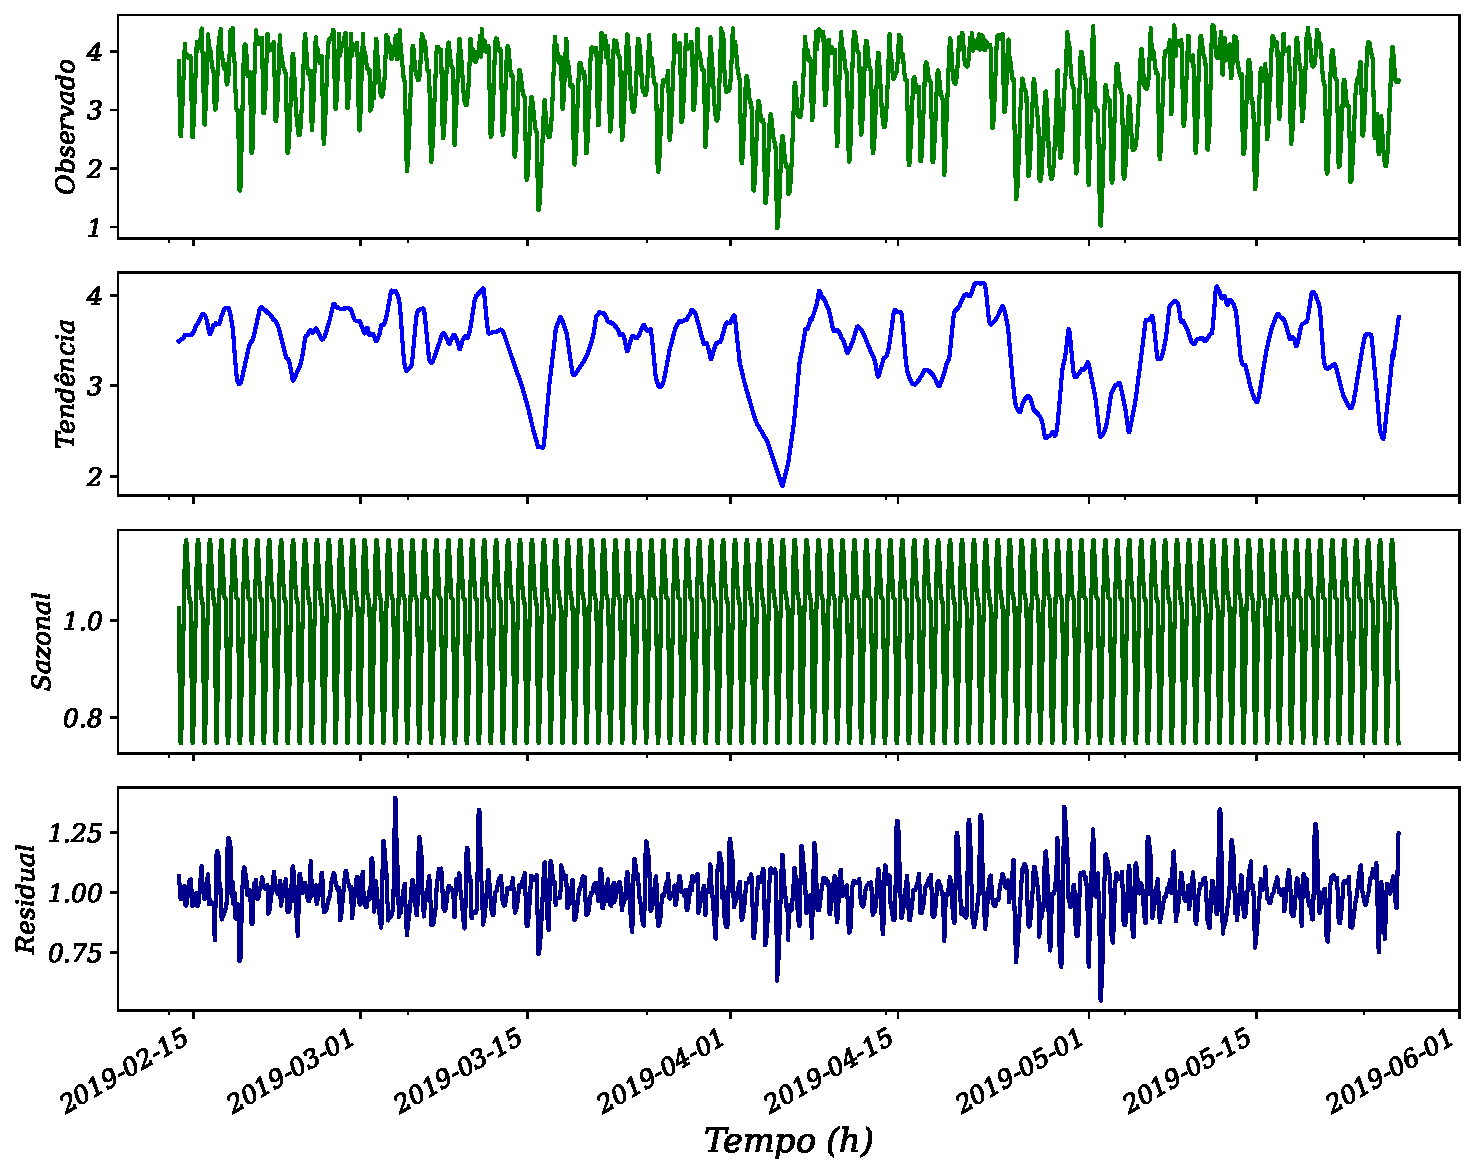
\includegraphics[width=\linewidth]{Resultados/Figuras/STL}
		\caption{Decomposição STL multiplicativa dos dados coletados}
		\label{fig:stl}
	\end{subfigure}
	
	\fonte{Elaboração própria a partir de dados da SANEPAR (2018 a 2020)}
\end{figure}

Na resposta à pergunta \ref{q5}\ref{q5:b}, as Figuras \ref{fig:stl-aditiva} e \ref{fig:stl} fornecem informações sobre a presença de tendência, sazonalidade e resíduos na série temporal.

Através da decomposição, é possível analisar se a série apresenta tendência, sazonalidade e resíduos. Ao observar as Figuras \ref{fig:stl-aditiva} e \ref{fig:stl}, é evidente que os dados exibem ambos os padrões. Isso indica que a série é estacionária, como confirmado pelo seguinte teste.

Teste de Dickey-Fuller (DF) Aumentado:
\begin{itemize}
	\item Estatística de teste ADF: $-4,25$
	\item Valor de p: $0,001$
	\item Atrasos utilizados: $21$
	\item Observações: $1074$
	\item Valor crítico ($1\%$): $-3,44$
	\item Valor crítico ($5\%$): $-2,86$
	\item Valor crítico ($10\%$): $-2,57$
\end{itemize}

Com base na forte evidência contra a hipótese nula, podemos rejeitar a hipótese nula. Isso indica que os dados não possuem raiz unitária e são estacionários em \ref{q5}\ref{q5:c}. Identificar as horas de pico entre 18h e 21h não é uma tarefa fácil. No entanto, ao observar a Figura \ref{fig:hist}, podemos notar um aumento na demanda durante essas horas durante o ano de 2020.
	
	
	\begin{figure}[!htb]
		\centering
		\caption{Violino no nível do reservatório}
		\label{fig:hist}
		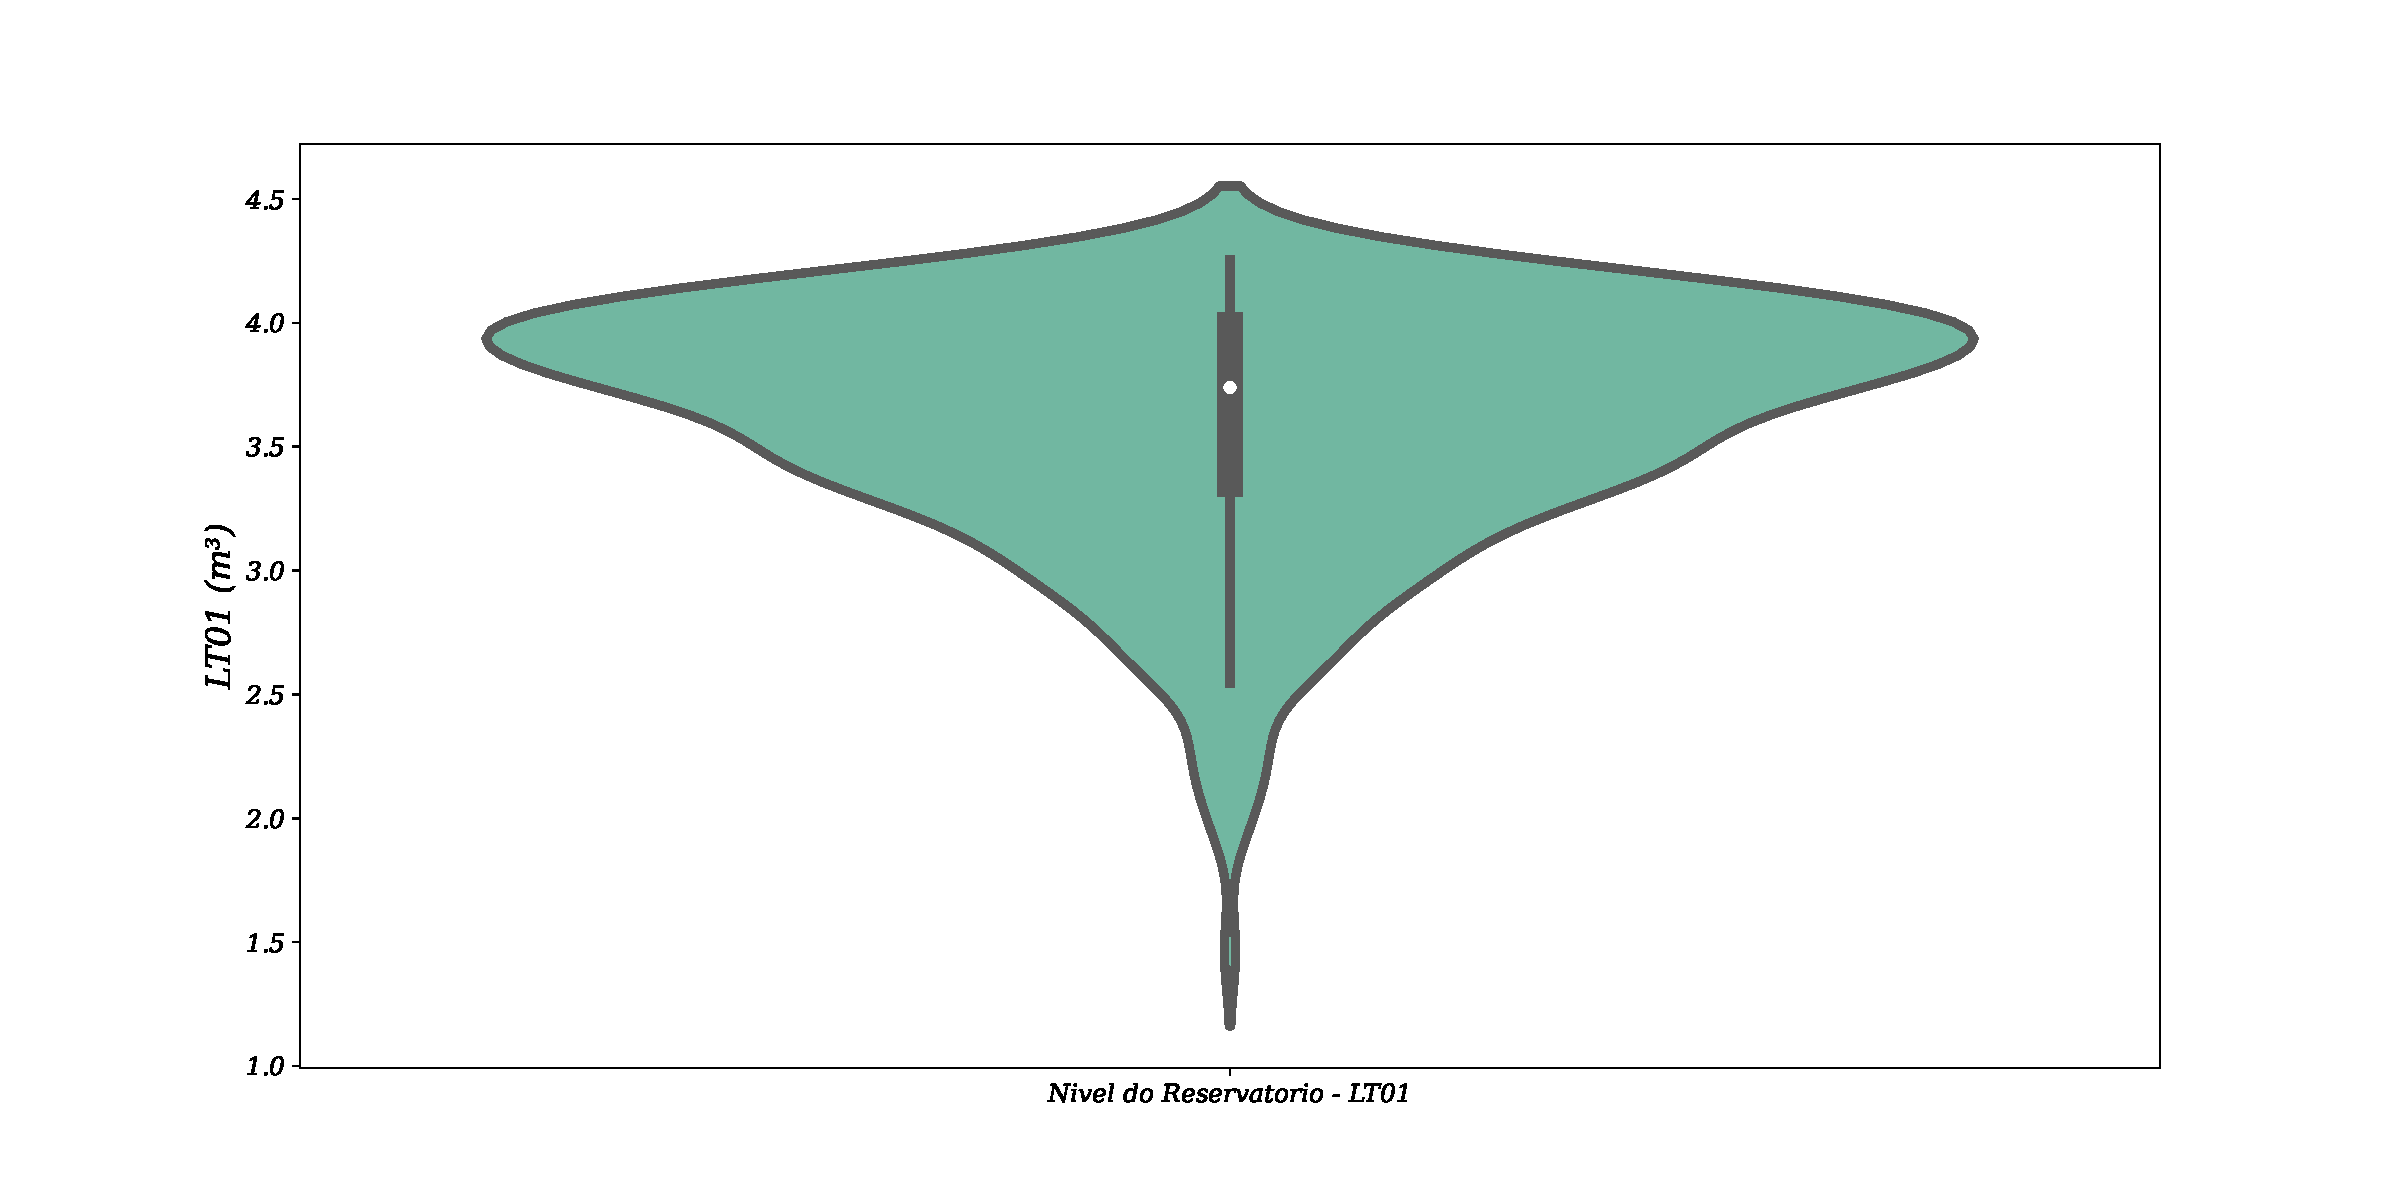
\includegraphics[width=0.9\linewidth]{Resultados/Figuras/viol}
		
		\fonte{Elaboração própria a partir de dados da SANEPAR (2018 a 2020)}
	\end{figure}
	
Conforme mencionado na subseção \ref{subsubsec:motivacao}, as anomalias climáticas ocorridas em 2020, especialmente a falta de chuvas, tiveram um impacto significativo nos resultados. Isso contribuiu para as mudanças observadas na demanda de água ao longo desse período.

Com relação à pergunta \ref{q5}\ref{q5:d}, durante as horas de pico, é necessário que o nível do tanque esteja dentro da faixa de $[3.545,4.256] m^3$ para evitar o acionamento das bombas. Manter o nível do tanque dentro dessa faixa permitirá que o sistema opere de forma eficiente, atendendo à demanda sem a necessidade de acionar as bombas.
	
	
	\begin{figure}[!htb]
		\centering
		\caption{Violino da vazão de recalque}
		\label{fig:ft03}
		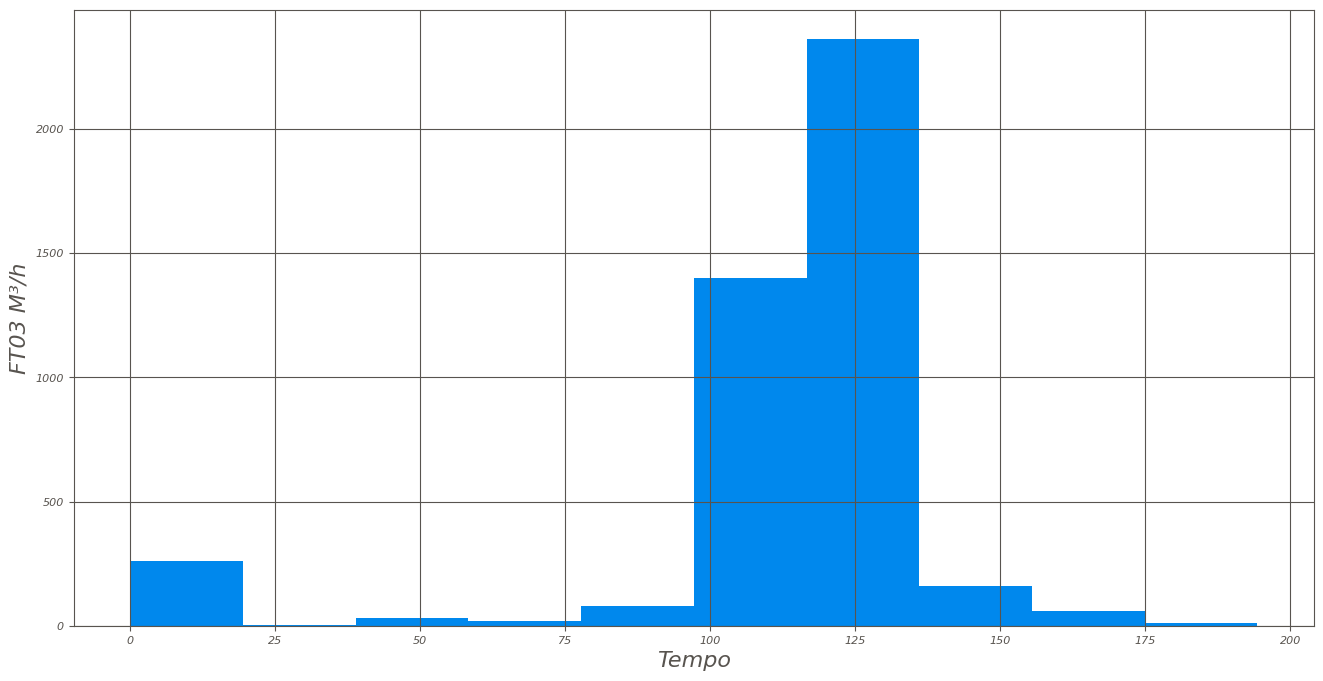
\includegraphics[width=0.9\linewidth]{Resultados/Figuras/ft03}
		
		\fonte{Elaboração própria a partir de dados da SANEPAR (2018 a 2020)}
	\end{figure}
	
Para responder à pergunta \ref{q5}\ref{q5:e}, a Figura \ref{fig:ft03} ilustra como a vazão pode ser afetada pelo nível do tanque. É interessante observar que a vazão de recalque tem um impacto mais significativo no nível do tanque em comparação com as outras vazões. Isso ocorre porque a vazão de recalque está associada à injeção de água diretamente no tanque por meio da bomba localizada próxima à base do tanque. Por outro lado, as demais vazões apresentam alguns valores ausentes, o que limita sua influência na análise geral.	
	


De acordo com o \citeonline{Reisen2017115}, o teste DF tem as seguintes equações

\begin{eqnarray}
	z_t&=& y_t+\theta \beta_t, \qquad t=1,\ldots, T, \label{eq:df3}\\	
	\hat{\rho}_{\mathrm{DF}}-1&=&\frac{\sum_{t=1}^T z_{t-1} \Delta z_t}{\sum_{t=1}^T z_{t-1}^2} \label{eq:regdf}
\end{eqnarray}

De \eqref{eq:regdf} onde $\Delta z_t=z_t-z_{t-1}$. Sob a hipótese nula $\left(H_0\right)$ : `` $\rho=1$'', as estatísticas do teste DF e suas distribuições limitantes são dadas da seguinte forma:


\begin{eqnarray}
	T\left(\hat{\rho}_{\mathrm{DF}}-1\right)=T \frac{\sum_{t=1}^T z_{t-1} \Delta z_t}{\sum_{t=1}^T z_{t-1}^2}
\end{eqnarray}
e


\begin{eqnarray}
	\hat{\tau}_{\mathrm{DF}}&=&\frac{\hat{\rho}_{\mathrm{DF}}-1}{\hat{\sigma}_{\mathrm{DF}}\left(\sum_{t=1}^T z_{t-1}^2\right)^{-1 / 2}} \label{eq:df}
\end{eqnarray}

De \eqref{eq:df} onde $\hat{\sigma}_{\mathrm{DF}}^2=T^{-1} \sum_{t=1}^T\left(\Delta z_t-\left(\hat{\rho}_{\mathrm{DF}}-1\right) z_{t-1}\right)^2 .$



Suponha que $\left(z_t\right)_{1 \leq t \leq T}$ são dadas por \eqref{eq:df3}, então quando $\rho=1$,


\begin{eqnarray}
	T\left(\hat{\rho}_{\mathrm{DF}}-1\right) \stackrel{d}{\longrightarrow} \frac{W(1)^2-1}{2 \int_0^1 W(r)^2 \mathrm{~d} r}-\left(\frac{\theta}{\sigma}\right)^2 \frac{\pi}{\int_0^1 W(r)^2 \mathrm{~d} r}, \text { como } T \rightarrow \infty \\
	\hat{\tau}_{\mathrm{DF}} \stackrel{d}{\longrightarrow}\left[1+2(\theta / \sigma)^2 \pi\right]^{-1 / 2}\left\{\frac{W(1)^2-1}{2\left(\int_0^1 W(r)^2 \mathrm{~d} r\right)^{1 / 2}}-\frac{(\theta / \sigma)^2 \pi}{\left(\int_0^1 W(r)^2 \mathrm{~d} r\right)^{1 / 2}}\right\} \\
	\quad \operatorname{como} T \rightarrow \infty\label{eq:df2}
\end{eqnarray}

A partir de \eqref{eq:df2}, onde $\stackrel{d}{\longrightarrow}$ denota convergência na distribuição e onde $\left\{W(r), r \in[0,1]\right\}$ denota o movimento Browniano padrão.

O ACF (do inglês \textit{Auto-Correlation Function}) é uma medida estatística utilizada para identificar a presença de correlação serial em uma série temporal. Ele calcula a autocorrelação entre os valores da série em diferentes defasagens, ou seja, a correlação entre os valores atuais e os valores passados da série. 

O ACF é útil para analisar a dependência temporal dos dados e identificar padrões de sazonalidade, tendência ou outros efeitos temporais. Através do ACF, é possível avaliar se a série exibe autocorrelação significativa em defasagens específicas, o que pode indicar a presença de não estacionariedade ou estrutura temporal que precisa ser considerada na análise ou modelagem da série temporal.

\begin{figure}[!htb]
	\centering
	\caption{Autocorrelação e Autocorrelação parcial}
	\label{fig:acf}
	
	
	\begin{subfigure}{0.9\textwidth}
		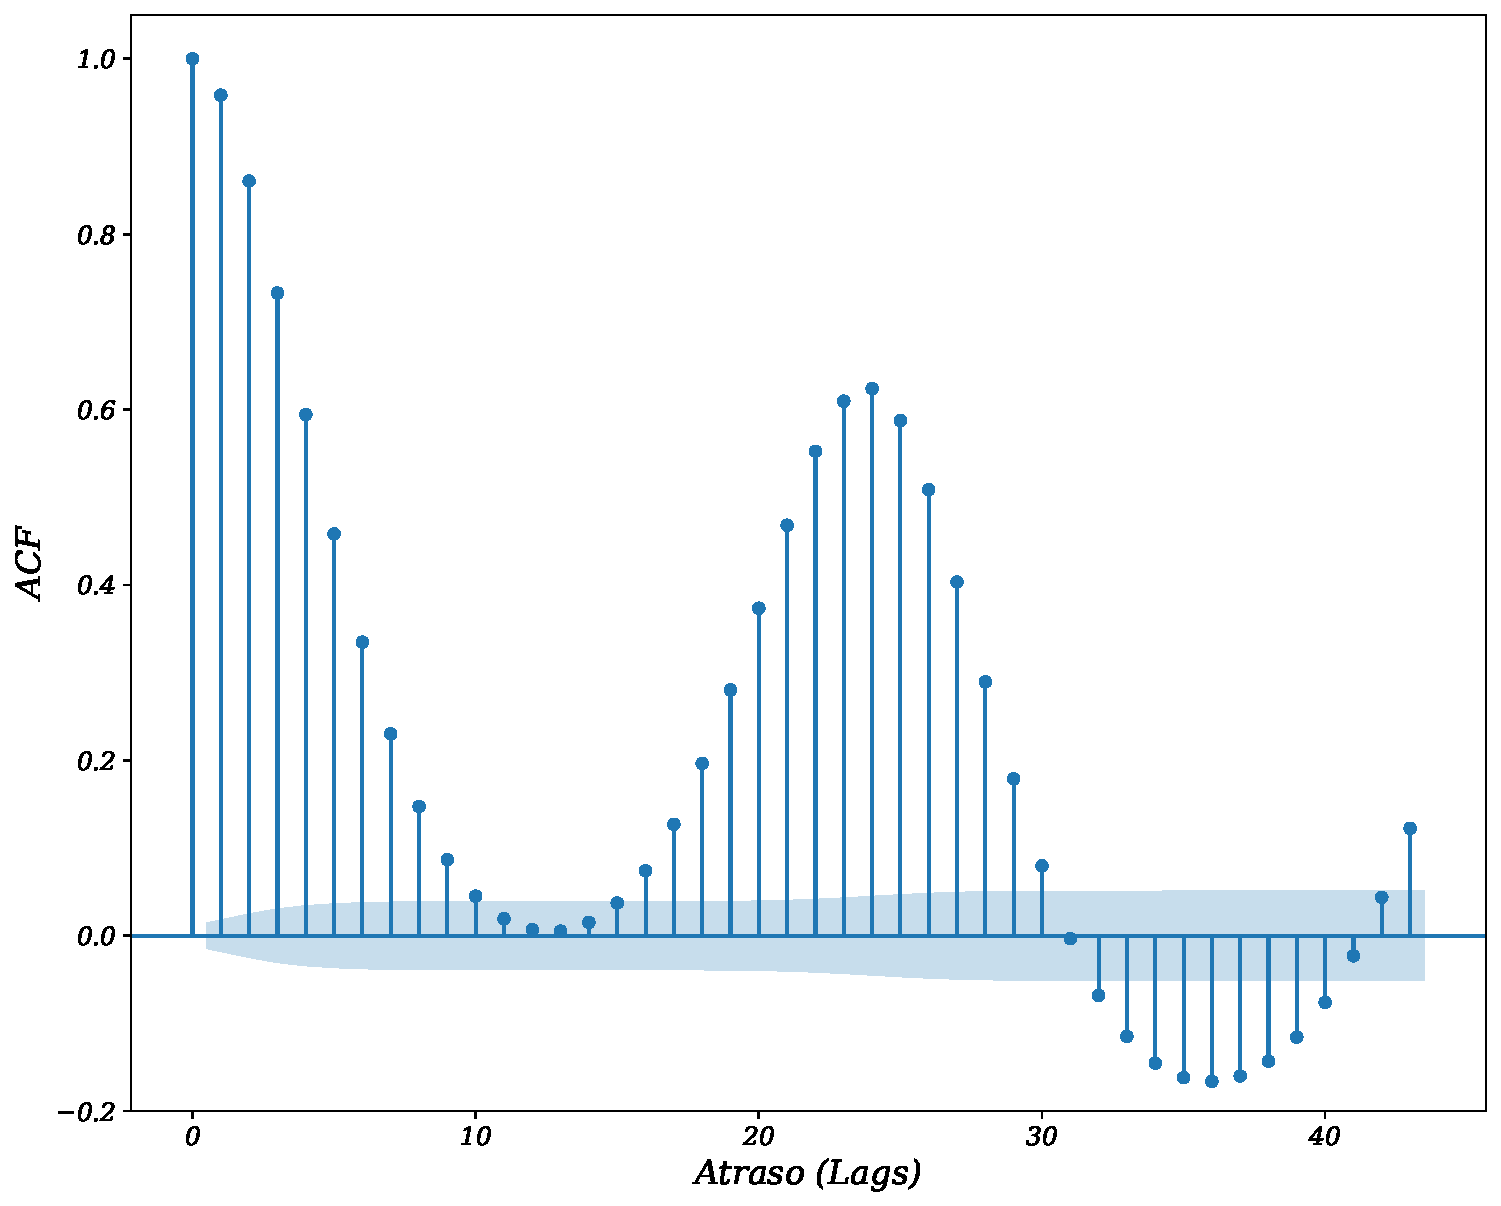
\includegraphics[width=\linewidth]{Resultados/Figuras/acf} 
		\caption{ACF}\label{fig:acfa}
	\end{subfigure}
	

	\begin{subfigure}{0.9\textwidth}
		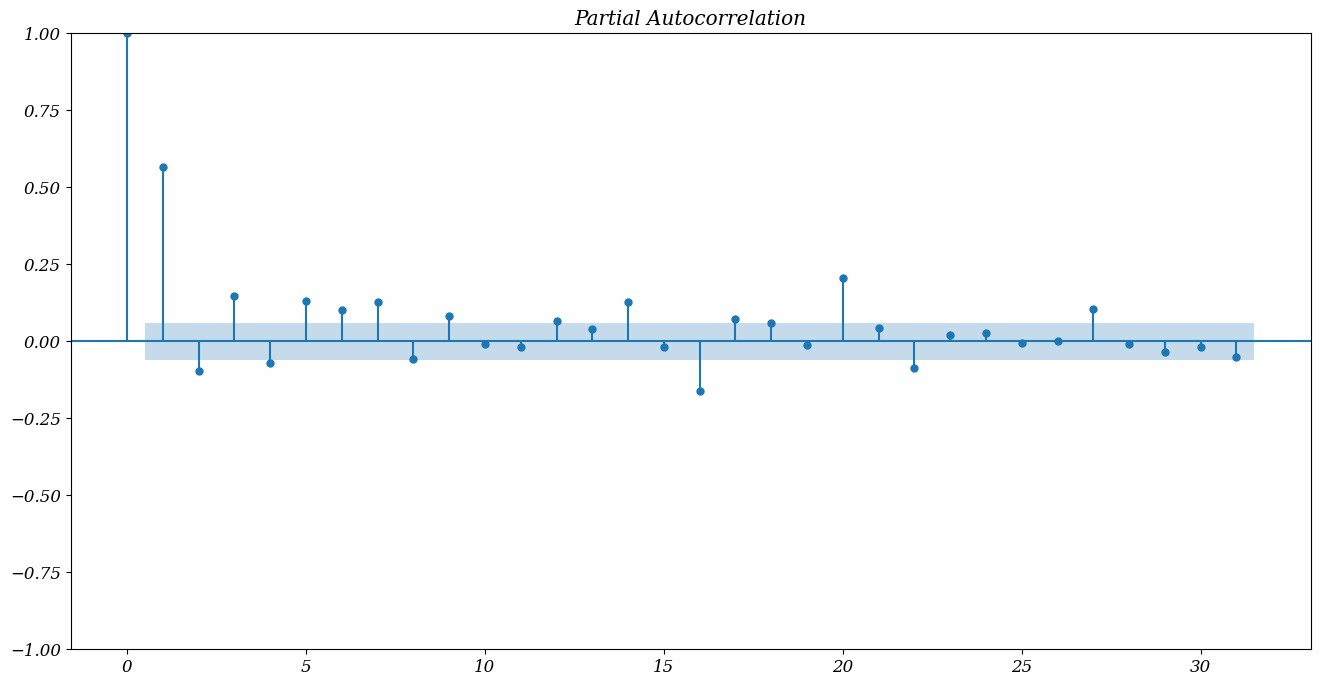
\includegraphics[width=\linewidth]{Resultados/Figuras/pacf}
		\caption{PACF}\label{fig:pacf}
	\end{subfigure}
	
	\fonte{Elaboração própria a partir de dados da SANEPAR (2018 a 2020)}
\end{figure}

A estatística ADF (do ingê \textit{Augmented Dickey-Fuller}) de $-4,27$ indica a evidência de estacionariedade na série temporal. Quanto mais negativo for o valor da estatística ADF, maior é a evidência de estacionariedade nos dados.

O valor-p de $0,0005$, por sua vez, está associado ao teste ADF. O valor-p é uma medida estatística que representa a probabilidade de obter um resultado igual ou mais extremo do que o observado, sob a suposição de que a hipótese nula seja verdadeira. No caso do teste ADF, a hipótese nula é a presença de raiz unitária na série temporal, o que indica não estacionariedade. Assim, um valor-p baixo (geralmente abaixo de um nível de significância predefinido, como 0,05) sugere que a série temporal é estacionária, enquanto um valor-p alto sugere que a série temporal é não estacionária. Neste caso, o valor-p de $0,0005$ é bastante baixo, o que indica forte evidência contra a hipótese nula e sugere que a série temporal é estacionária.

Na Figura \ref{fig:acf}, pode-se observar a diferença entre a autocorrelação (ACF) exibida na Figura \ref{fig:acfa} e a autocorrelação parcial (PACF) exibida na Figura \ref{fig:pacf}. A autocorrelação é uma medida da correlação entre os valores da série temporal em diferentes defasagens, levando em consideração tanto a correlação direta quanto a correlação indireta. Por outro lado, a autocorrelação parcial mede apenas a correlação direta entre os valores, desconsiderando a influência das defasagens intermediárias. Essas análises são úteis para identificar padrões e relações de dependência entre os valores da série temporal, fornecendo informações importantes para a modelagem e previsão desses dados.

O intervalo de confiança padrão de 95\% é representado pela marca azul na Figura. As observações que estão fora desse intervalo são consideradas estatisticamente correlacionadas, indicando a presença de padrões ou estrutura na série temporal.

A correlação visualizada na Figura \ref{fig:acf} é fundamental para a interpretação do teste DF. Em uma série de ruído branco, os valores são completamente aleatórios e não apresentam correlação significativa. Portanto, quando há correlação presente na série, isso indica a existência de padrões ou dependências entre os valores, o que pode ser explorado para a modelagem e previsão da série temporal.

\begin{figure}[!htb]
	\centering
	\caption{Ruído branco}
	\label{fig:ruido-branco}
	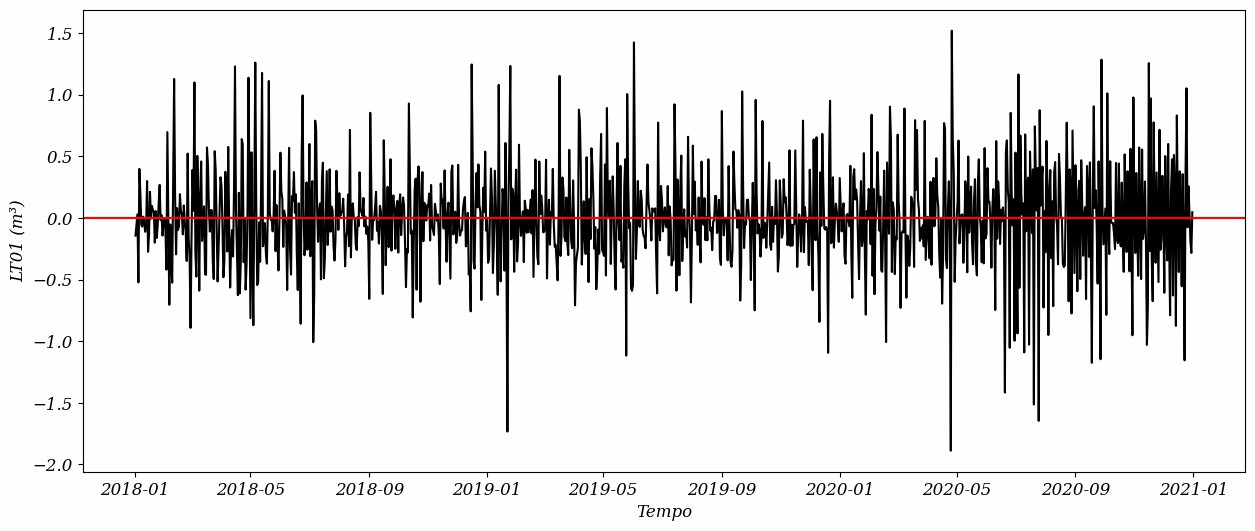
\includegraphics[width=0.9\linewidth]{Resultados/Figuras/ruido-branco}
	
	\fonte{Elaboração própria a partir de dados da SANEPAR (2018 a 2020)}
\end{figure}

Na Figura \ref{fig:ruido-branco}, é possível observar uma série temporal que pode ser caracterizada como ruído branco. Uma série temporal é considerada ruído branco se suas variáveis forem independentes e distribuídas de forma idêntica, com média zero. Isso implica que todas as variáveis possuem a mesma variância ($\sigma^2$) e que cada valor não possui correlação com os demais valores da série.

Além disso, é importante destacar o comprimento dos zeros na variável prevista, o que conclui a etapa \ref{etp:3}.

\subsubsection{Separa\c c\~ao dos dados}\label{subsubsec:divisao}

Na etapa \ref{etp:4}, os dados foram divididos em conjuntos de treinamento, teste e validação. Essa prática é comum entre profissionais de aprendizado de máquina, pois permite avaliar o desempenho do modelo em conjuntos de dados diferentes.

Em relação ao processamento de modelos de aprendizado profundo, é importante mencionar as inovações trazidas pela empresa Nvidia ao longo dos anos, especialmente no campo do processamento de imagens. O lançamento da placa de vídeo GeForce RTX 4090 tem sido bastante aguardado tanto por gamers quanto por profissionais que lidam com aprendizado de máquina.

No contexto do estudo, foram utilizados dois computadores para realizar os cálculos dos modelos. Um deles é equipado com um processador Intel Core i5-3330 e o outro é um notebook com um processador Intel Core i7-5500. Ambos os processadores possuem 4 threads, sendo que o notebook possui 2 núcleos físicos e o i5 possui 4 núcleos físicos. Cada processador tem suas especificações e desempenho adequados a diferentes necessidades. Vale ressaltar que não é obrigatório utilizar as últimas gerações de processadores para realizar esses processamentos, e sim compreender e aplicar corretamente os recursos disponíveis.

Quanto à divisão dos dados, foi adotada uma estratégia básica em que 70\% dos dados foram destinados ao conjunto de treinamento e os 30\% restantes foram reservados para o conjunto de teste. Dentro dos 70\% de treinamento, foi realizada uma subdivisão em que 80\% desses dados foram usados novamente para treinamento e os 20\% restantes foram utilizados para validação. Essa abordagem foi implementada em linguagem de programação para facilitar o processo e evitar a necessidade de recalculá-la a cada modificação do modelo.

\subsubsection{Estrat\'egia de Previs\~ao}\label{subsubsec:est}

A estratégia recursiva é mencionada por \citeonline{PETROPOULOS2022705} como uma abordagem eficaz na previsão de séries temporais de múltiplos passos. De acordo com o autor, essa estratégia envolve o uso de previsões anteriores como entradas para prever os próximos passos da série temporal. A abordagem recursiva tem demonstrado potencial para melhorar a acurácia das previsões de séries temporais de longo prazo.

Na Etapa \ref{etp:5}, discute-se a previsão dos dados em uma janela de horizonte de previsão estendida, abrangendo diferentes períodos de tempo, como um dia, uma semana, duas semanas e um mês. Essa estratégia de previsão recorrente permite a comparação entre modelos de regressão e modelos ARIMA em diferentes horizontes temporais.

Essa abordagem é vantajosa, pois cada modelo possui suas próprias características e desempenho ao lidar com previsões de curto prazo, como um dia, e previsões de prazo mais longo, como um mês. Ao utilizar uma janela de previsão mais ampla, é possível observar e avaliar melhor as diferenças entre os modelos e analisar seu desempenho em horizontes de tempo variados.

\textbf{Validação e ajuste do modelo}
na etapa \ref{etp:6}, o horizonte de previsão foi personalizado com base no método recursivo de previsão de série temporal e na previsão do nível do tanque LT01. Foram selecionados os seguintes passos para a previsão à frente: uma hora, seis horas, doze horas e um dia. Essa escolha do horizonte de previsão foi feita levando em consideração a estratégia recursiva e os objetivos específicos do estudo. Identifica-se que essa janela de tempo proporciona uma análise mais adequada e comparável entre os modelos utilizados.

Foram utilizados os parâmetros obtidos pelo autoARIMA, que são $(p = 7, d = 0, q = 0) (P = 2, D = 1, Q = 1)_{M = 12}$, mas foram ajustados para obter um melhor resultado, sendo $(p = 7, d = 1, q = 7) (P = 2, D = 1, Q = 1)_{M = 12}$. Na Tabela \ref{tab:autoarima_params}, são exibidos todos os modelos obtidos por esse método do ``autoARIMA'' e ajustados para que obtenham o melhor resultado.
\(p\): Ordem do componente AR (\textit{Auto-Regressivo}),
\(d\): Número de diferenciações não sazonais,
\(q\): Ordem do componente MA (\textit{Média Móvel}),
\(P\): Ordem do componente AR sazonal,
\(D\): Número de diferenciações sazonais,
\(Q\): Ordem do componente MA sazonal,
\(M\): Período sazonal (número de observações em um ciclo sazonal).
Na Tabela \ref{tb:resltsar} mostra como a biblioteca do Python autoARIMA obteve os resultados dos parâmetros, exibindo o STD e os intervalos de confiança nos quais o modelo alcançou o melhor desempenho. O leve ajuste realizado não altera significativamente os parâmetros obtidos nesta biblioteca, permitindo que cada modelo seja trabalhado de maneira eficiente.

\begin{table}[!htb]
	\centering
	\caption{Parâmetros utilizados nos modelos ARIMA e seus antecessores obtidos pelo ``autoARIMA'' do Python.}
	\label{tab:autoarima_params}
	\small
	\begin{tabular}{
			>{\centering\arraybackslash}p{5.5cm}
			>{\centering\arraybackslash}p{6cm}
			>{\centering\arraybackslash}p{3cm}
		}
		\toprule
		\textbf{Modelo} & \textbf{Parâmetros Utilizados} & \textbf{Método de Estimação} \\
		\midrule
		AR(p) & \( p = 7 \) & AutoARIMA \\
		ARX(p) & \( p = 7 \) & AutoARIMA \\
		MA(q) & \( q = 7 \) & AutoARIMA  \\
		ARMA(p, q) & \( p = 7 \), \( q = 7 \) & AutoARIMA  \\
		ARIMA(p, d, q) & \( p = 7 \), \( d = 1 \), \( q = 7 \) & AutoARIMA  \\
		ARIMAX(p, d, q) & \( p = 7 \), \( d = 1 \), \( q = 7 \) & AutoARIMA  \\
		SARIMA(p, d, q)(P, D, Q) & \( p = 7 \), \( d = 1 \), \( q = 7 \), \( P = 2 \), \( D = 1 \), \( Q = 1 \), \( M = 12 \) & AutoARIMA  \\
		SARIMAX(p, d, q)(P, D, Q, M) & \( p = 7 \), \( d = 1 \), \( q = 7 \), \( P = 2 \), \( D = 1 \), \( Q = 1 \), \( M = 12 \) & AutoARIMA  \\
		\bottomrule
	\end{tabular}
\end{table}



\begin{table}[!htb]
	\centering
	\caption{SARIMAX$(7, 0, 0)\times(2, 1, [1], 12)$ Results} \label{tb:resltsar}
	\begin{tabular}{
			l
			S[table-format=1.4]
			S[table-format=1.4]
			S[table-format=3.3]
			S[table-format=1.3]
			S[table-format=1.3]
			S[table-format=1.3]
		}
		\toprule
		& {Coef} & {STD Err} & {z} & {P$>|z|$} & {[0,025} & {0,975]} \\
		\midrule
		Intercept & 0,0003 & 0,000 & 1,053 & 0,292 & -0,000 & 0,001 \\
		ar.L1 & 1,6149 & 0,011 & 141,865 & 0,000 & 1,593 & 1,637 \\
		ar.L2 & -0,8879 & 0,021 & -42,045 & 0,000 & -0,929 & -0,847 \\
		ar.L3 & 0,3167 & 0,024 & 13,033 & 0,000 & 0,269 & 0,364 \\
		ar.L4 & -0,1056 & 0,027 & -3,961 & 0,000 & -0,158 & -0,053 \\
		ar.L5 & -0,1099 & 0,028 & -3,928 & 0,000 & -0,165 & -0,055 \\
		ar.L6 & 0,1431 & 0,027 & 5,368 & 0,000 & 0,091 & 0,195 \\
		ar.L7 & -0,0673 & 0,015 & -4,583 & 0,000 & -0,096 & -0,039 \\
		ar.S.L12 & -0,1222 & 0,016 & -7,705 & 0,000 & -0,153 & -0,091 \\
		ar.S.L24 & 0,1692 & 0,014 & 12,244 & 0,000 & 0,142 & 0,196 \\
		ma.S.L12 & -0,8728 & 0,012 & -74,569 & 0,000 & -0,896 & -0,850 \\
		sigma2 & 0,0157 & 0,000 & 60,022 & 0,000 & 0,015 & 0,016 \\
		\bottomrule
	\end{tabular}
\end{table}


Para os modelos de gradiente \textit{boosting} e redes neurais artificiais, os hiperparâmetros foram otimizados usando a biblioteca Optuna do Python. Nesse contexto, são empregadas técnicas bayesianas, especificamente o algoritmo TPE, visando uma otimização mais eficiente.

Os modelos XGBoost e LightGBM tem como parâmetros e hiperparâmetros mostrado na Tabela \ref{tab:hiperparametros} a otimização dos paramétrios dos modelos XGBoost, LightGBM, RFR e DTR. Esses modelos, devido à sua semelhança, exibem tempos de desempenho próximos um do outro. 



\begin{table}[!htb]
	\centering
	\caption{Hiperparâmetros dos modelos}
	\label{tab:hiperparametros}
	\begin{tabular}{
			>{\centering\arraybackslash}p{2.2cm}
			>{\centering\arraybackslash}p{2.8cm}
			>{\centering\arraybackslash}p{1.9cm}
			>{\centering\arraybackslash}p{1.9cm}
			>{\centering\arraybackslash}p{1.9cm}
			>{\centering\arraybackslash}p{1.9cm}
			>{\centering\arraybackslash}p{1.9cm}
		}
		\toprule
		\textbf{Modelo} & \textbf{Estimadores} & \textbf{Profund. Máxima} & \textbf{Min. Amostras Divisão} & \textbf{Min. Amostras por Folha} & \textbf{Máx. Recursos} & \textbf{Taxa de Aprendizado} \\
		\midrule
		XGB Regressor & 503 & 5 & 7 & 2 & ``sqrt'' & 0,034 \\
		LGBM Regressor & 820 & 10 & 3 & 5 & ``auto'' & 0,014 \\
		Random Forest Regressor & 135 & 10 & 4 & 2 & None & N/A \\
		Decision Tree Regressor & N/A & 229 & 32 & 20 & None & N/A \\
		\bottomrule
	\end{tabular}
\end{table}



Os modelos de rede neural artificial, como RNN, ANN, CNN, GRU, LSTM e Transformer, obtidos na otimização do Optuna do Python, tiveram seus hiperparâmetros melhorados, conforme exibido na Tabela \ref{tab:hyperparameters_summary}. Esses modelos, por serem modelos de rede neural artificial, são melhores para otimizar do que os outros. 

\begin{table}[!htb]
	\centering
	\caption{Resumo dos Hiperparâmetros dos Modelos de Redes Neurais}
	\label{tab:hyperparameters_summary}
	\small
	\begin{tabular}{
			>{\centering\arraybackslash}p{1.8cm}
			>{\centering\arraybackslash}p{2cm}
			>{\centering\arraybackslash}p{2cm}
			>{\centering\arraybackslash}p{2cm}
			>{\centering\arraybackslash}p{2cm}
			>{\centering\arraybackslash}p{1.5cm}
			>{\centering\arraybackslash}p{2.5cm}
		}
		\toprule
		\textbf{Modelo} & \textbf{Unidades/ Layers} & \textbf{Heads/ Dimensões} & \textbf{Tamanho do Batch} & \textbf{Épocas} & \textbf{Dropout/ Learning Rate} & \textbf{Outros Parâmetros} \\
		\midrule
		LSTM & 128 & -- & 32 & 77 & -- & -- \\
		
		GRU & -- & -- & 32 & 50 & -- & -- \\
		
		Transformers & -- & 8 heads, 217; 433 & -- & 50 & -- & 2 camadas \\
		
		RNN & 79 & -- & 16 & 50 & 0,0008612 & -- \\
		
		CNN & -- & -- & 61 & 10 & 0,2799; 0,00052 & Kernel: 7, Densas: 1, Verbosidade: 1 \\
		
		ANN & 125 & -- & 27 & 96 & 0,4135, 0,0004057 & Densas: 1, Verbosidade: 0 \\
		\bottomrule
	\end{tabular}
\end{table}



\subsubsection{Modelos de previs\~ao e m\'etricas de desempenho}\label{subsubsec:modelos}

A partir da etapa \ref{etp:7}, foram utilizadas três métricas amplamente empregadas na literatura para a previsão e comparação de modelos ARIMA e modelos de regressão. Essas métricas foram detalhadas na seção \ref{subsec:metrica}.

Ao analisar os modelos desenvolvidos, foi observado que o modelo de regressão linear (LR) obteve o melhor desempenho tanto na previsão de curto prazo, considerando uma modelagem de 24 horas, quanto nas horas de pico entre 18h e 21h. Os modelos MA, AR, SARIMA, ARIMA, SARIMAX, ARIMAX, ARX, LGBMRegressor, XGBRegressor e RFR também apresentaram um desempenho satisfatório, seguindo uma ordem de melhor para pior.

Para previsões de longo prazo, como no caso dos 30 dias, foram avaliados os modelos ARMA, AR, MA, ARIMA, ARIMAX, ARX, SARIMA, SARIMA, XGBRegressor, RFR, LGBMRegressor e LR, novamente seguindo a ordem de melhor desempenho. No entanto, ao analisar os resultados graficamente nos apêndices, foi observado que os modelos que incorporam variáveis exógenas parecem ter uma capacidade de previsão superior em relação aos demais modelos. Essa tendência pode ser visualizada nas Figuras de \ref{fig:1-AR-ARX-MA24} a \ref{fig:60-ARIMAX-SARIMA-SARIMAX24} e nas Tabelas de \ref{tb:1-24trn} a \ref{tb:60-24cm}.


\subsubsection{Relat\'orio dos Resultados}

Na etapa \ref{etp:9}, foi utilizado o teste de Friedman e Nemenyi para comparar as classificações médias entre os classificadores. O teste de Nemenyi é um teste de comparação múltipla utilizado após a aplicação de testes não paramétricos com três ou mais fatores.

\begin{table}[!htb]
	\centering
	\caption{Teste Nemenyi}
	\begin{tabular}{@{}clllllllll@{}}
		\toprule
		\multicolumn{1}{l}{\textbf{Nemenyi}} & \multicolumn{1}{c}{\textbf{0}} & \multicolumn{1}{c}{\textbf{1}} & \multicolumn{1}{c}{\textbf{2}} & \multicolumn{1}{c}{\textbf{3}} & \multicolumn{1}{c}{\textbf{4}} & \multicolumn{1}{c}{\textbf{5}} & \multicolumn{1}{c}{\textbf{6}} & \multicolumn{1}{c}{\textbf{7}} & \multicolumn{1}{c}{\textbf{8}} \\ \midrule
		\textbf{0}                           & 1,000                          & 0,001                          & 0,001                          & 0,001                          & 0,001                          & 0,001                          & 0,001                          & 0,001                          & 0,001                          \\
		\textbf{1}                           & 0,001                          & 1,000                          & 0,001                          & 0,001                          & 0,001                          & 0,001                          & 0,001                          & 0,001                          & 0,157                          \\
		\textbf{2}                           & 0,001                          & 0,001                          & 1,000                          & 0,847                          & 0,001                          & 0,001                          & 0,001                          & 0,001                          & 0,001                          \\
		\textbf{3}                           & 0,001                          & 0,001                          & 0,847                          & 1,000                          & 0,001                          & 0,001                          & 0,001                          & 0,001                          & 0,001                          \\
		\textbf{4}                           & 0,001                          & 0,001                          & 0,001                          & 0,001                          & 1,000                          & 0,001                          & 0,001                          & 0,001                          & 0,001                          \\
		\textbf{5}                           & 0,001                          & 0,001                          & 0,001                          & 0,001                          & 0,001                          & 1,000                          & 0,001                          & 0,001                          & 0,001                          \\
		\textbf{6}                           & 0,001                          & 0,001                          & 0,001                          & 0,001                          & 0,001                          & 0,001                          & 1,000                          & 0,001                          & 0,001                          \\
		\textbf{7}                           & 0,001                          & 0,001                          & 0,001                          & 0,001                          & 0,001                          & 0,001                          & 0,001                          & 1,000                          & 0,001                          \\
		\textbf{8}                           & 0,001                          & 0,157                          & 0,001                          & 0,001                          & 0,001                          & 0,001                          & 0,001                          & 0,001                          & 1,000                          \\ \bottomrule
	\end{tabular}
	
	\fonte{Elaboração própria a partir de dados da SANEPAR (2018 a 2020)}
\end{table}

Para calcular a estatística de teste $F_r$ de Friedman, inicialmente cria-se uma tabela com os dados, onde cada linha representa uma amostra e cada coluna representa uma condição de teste. Em seguida, as amostras são ordenadas ao longo das condições, da melhor situação para a pior. Se não houver empates, a estatística de teste $F_r$ é calculada utilizando a seguinte fórmula:

\begin{equation}
	F_r = \left(\frac{12}{n k(k+1)} \sum_{i=1}^k R_i^2\right) - 3n(k+1)
\end{equation}

Nessa fórmula, $n$ é o número de linhas (ou amostras), $k$ é o número de colunas (ou condições) e $R_i$ é a soma das fileiras da coluna (ou condição) $i$.

Além disso, o valor crítico CD (Critical Difference) é utilizado para determinar se dois classificadores são significativamente diferentes um do outro. O CD é calculado usando a fórmula que mencionei anteriormente:

\begin{equation}
	CD = q_\alpha \sqrt{\frac{k(k+1)}{6N}}
\end{equation}

Na fórmula do CD, $q_\alpha$ é o valor crítico obtido da tabela de teste de Nemenyi, $k$ é o número de classificadores e $N$ é o número total de amostras.

De acordo com essa equação, os resultados da pesquisa foram os seguintes:

$statistic=8015.611,\ \ p-value=0.0$ com um total de 26.306 linhas por 9 colunas.


\subsubsection{Compara\c c\~ao dos Modelos}

Com o objetivo de obter uma análise mais aprofundada do desempenho de cada modelo, foi realizada uma comparação por meio de um gráfico de violino. Dessa forma, pôde-se observar qual dos modelos apresentava o melhor desempenho.



Ao examinar os modelos representados nas Figuras \ref{fig:modelos-arima} e \ref{fig:violin-lr-xgb-lgbm-rf}, identifico os modelos que se destacam em relação à natureza dos dados. Na Figura \ref{fig:basic_comparar}, que compara os modelos ARIMA e XGBoost com outros, torna-se evidente que os modelos ARIMA como AR, ARX, MA, ARMA, ARIMAX e SARIMAX demonstram um desempenho sólido. Além disso, os modelos baseados em gradientes e regressão, como o XGBoost, exibem resultados comparáveis, beneficiando-se da otimização por meio do Optuna, uma abordagem mais eficaz em relação aos tradicionais Grid Search e Randomized Search.

Na Figura \ref{fig:rrmse_comparar}, que contrasta as redes neurais com o modelo Prophet, é importante destacar que os modelos de redes neurais, incluindo RNN, LSTM, GRU, ANN, CNN e Transformer, foram avaliados em conjunto com o modelo Prophet. A análise estatística também demonstrou que o modelo RNN se sobressai como o vencedor entre as métricas avaliadas. Essa conclusão é respaldada pelas evidências de que pelo menos um modelo é superior aos demais. Os modelos com valores de p-valor abaixo de 0,05 foram realçados em \textit{itálico} para enfatizar sua significância.

A avaliação da eficácia dos modelos ARIMA em previsões de longo prazo emprega o teste de Ljung-Box, conforme detalhado no Apêndice \ref{sec:comtb18}. As Tabelas \ref{tb:lbtrn} a \ref{tb:lbcm} ilustram a acurácia dos modelos ARIMA ao longo do tempo, com valores menores sendo destacados em \textbf{negrito} e \textit{itálico} para facilitar a interpretação. Modelos como ARX, ARIMAX e SARIMAX, que incorporam variáveis exógenas, demonstram um desempenho superior nesse contexto. Esses modelos não lineares apresentam uma capacidade de previsão robusta em horizontes temporais mais longos, diferenciando-se positivamente dos outros modelos ARIMA. Na Figura \ref{fig:modelos-arima}, são selecionados os modelos ARIMA e seus antecessores. Esses modelos têm suas limitações, tanto para horizontes de previsão de curto prazo quanto para horizontes de longo prazo. Nessa comparação no gráfico de violino, são combinados vários outros gráficos em um só, como o gráfico de barras e o boxplot. Esse gráfico pode fornecer várias informações, mas o objetivo aqui é identificar apenas o melhor modelo entre os modelos ARIMA.
Como essa série não apresentou uma estacionariedade bem definida e os dados não a tornaram estacionária, os modelos que não têm sazonalidade mostraram-se superiores, tais como AR, MA, ARX, ARMA, ARIMA e ARIMAX. O modelo ARIMAX demonstrou ser bastante robusto para este caso, mas mesmo assim, modelos mais básicos como AR e MA ainda apresentaram resultados melhores.

\begin{figure}[H]
	\centering
	\caption{Comparação dos modelos ARIMA}\label{fig:modelos-arima}
	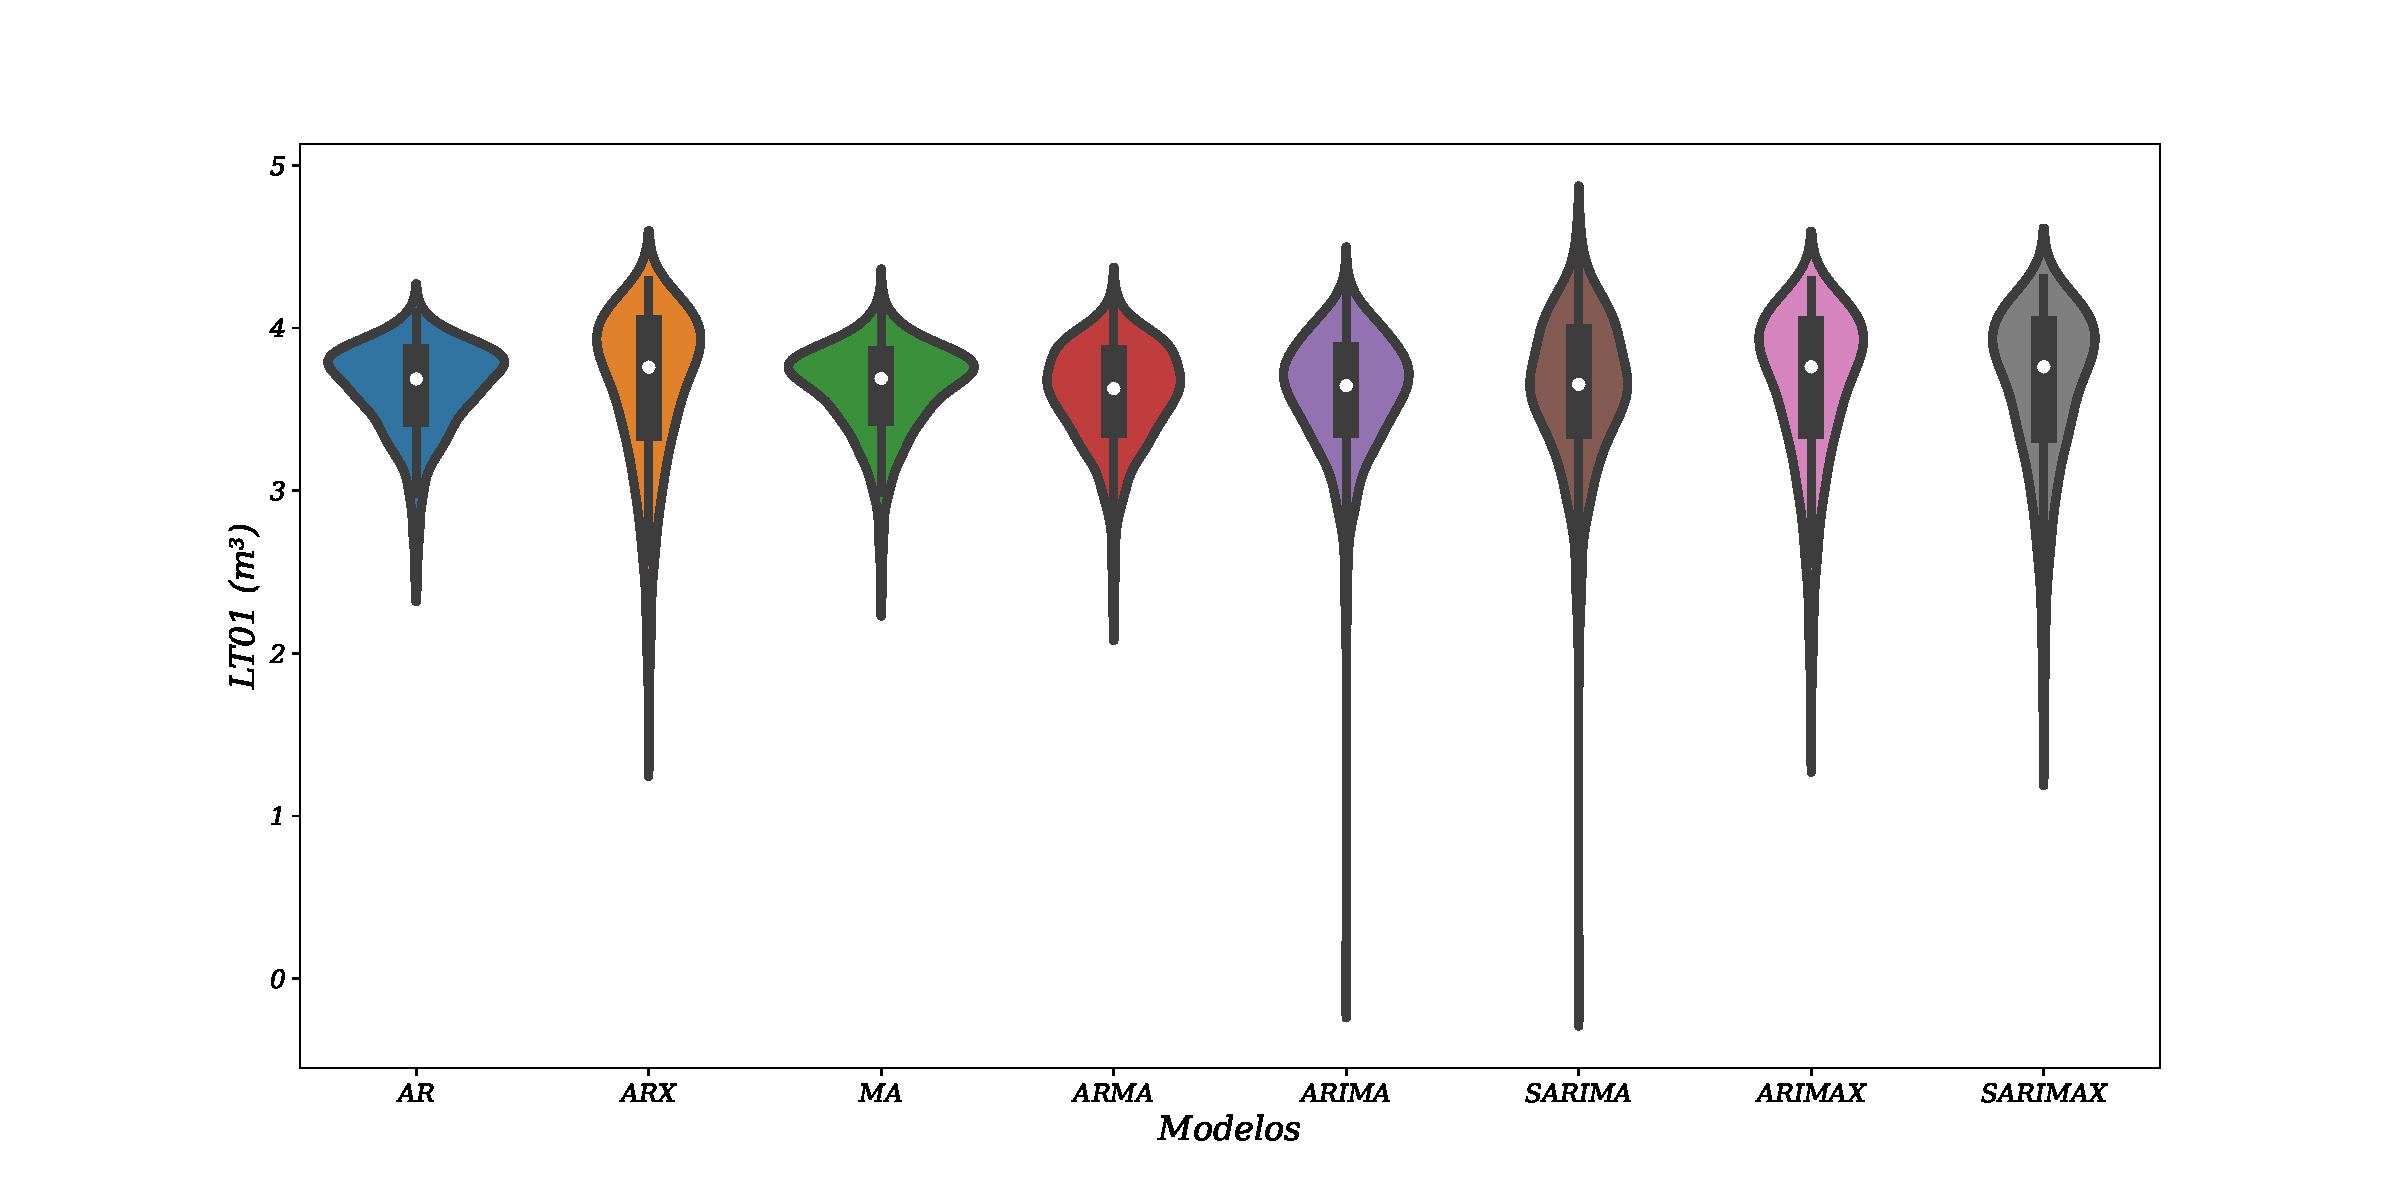
\includegraphics[width=1\linewidth]{Resultados/Figuras/modelos-arima}
	

\end{figure}

Na Figura \ref{fig:violin-lr-xgb-lgbm-rf}, é feita uma comparação entre os modelos de gradiente e regressor. Esses modelos, por serem mais robustos e utilizar técnicas de otimização mais avançadas, mostram-se superiores aos modelos comparados. O modelo XGBoost, em particular, é identificado como superior em relação aos outros modelos na análise.

\begin{figure}[H]
	\centering
	\caption{Comparação de modelos de regressão}\label{fig:violin-lr-xgb-lgbm-rf}
	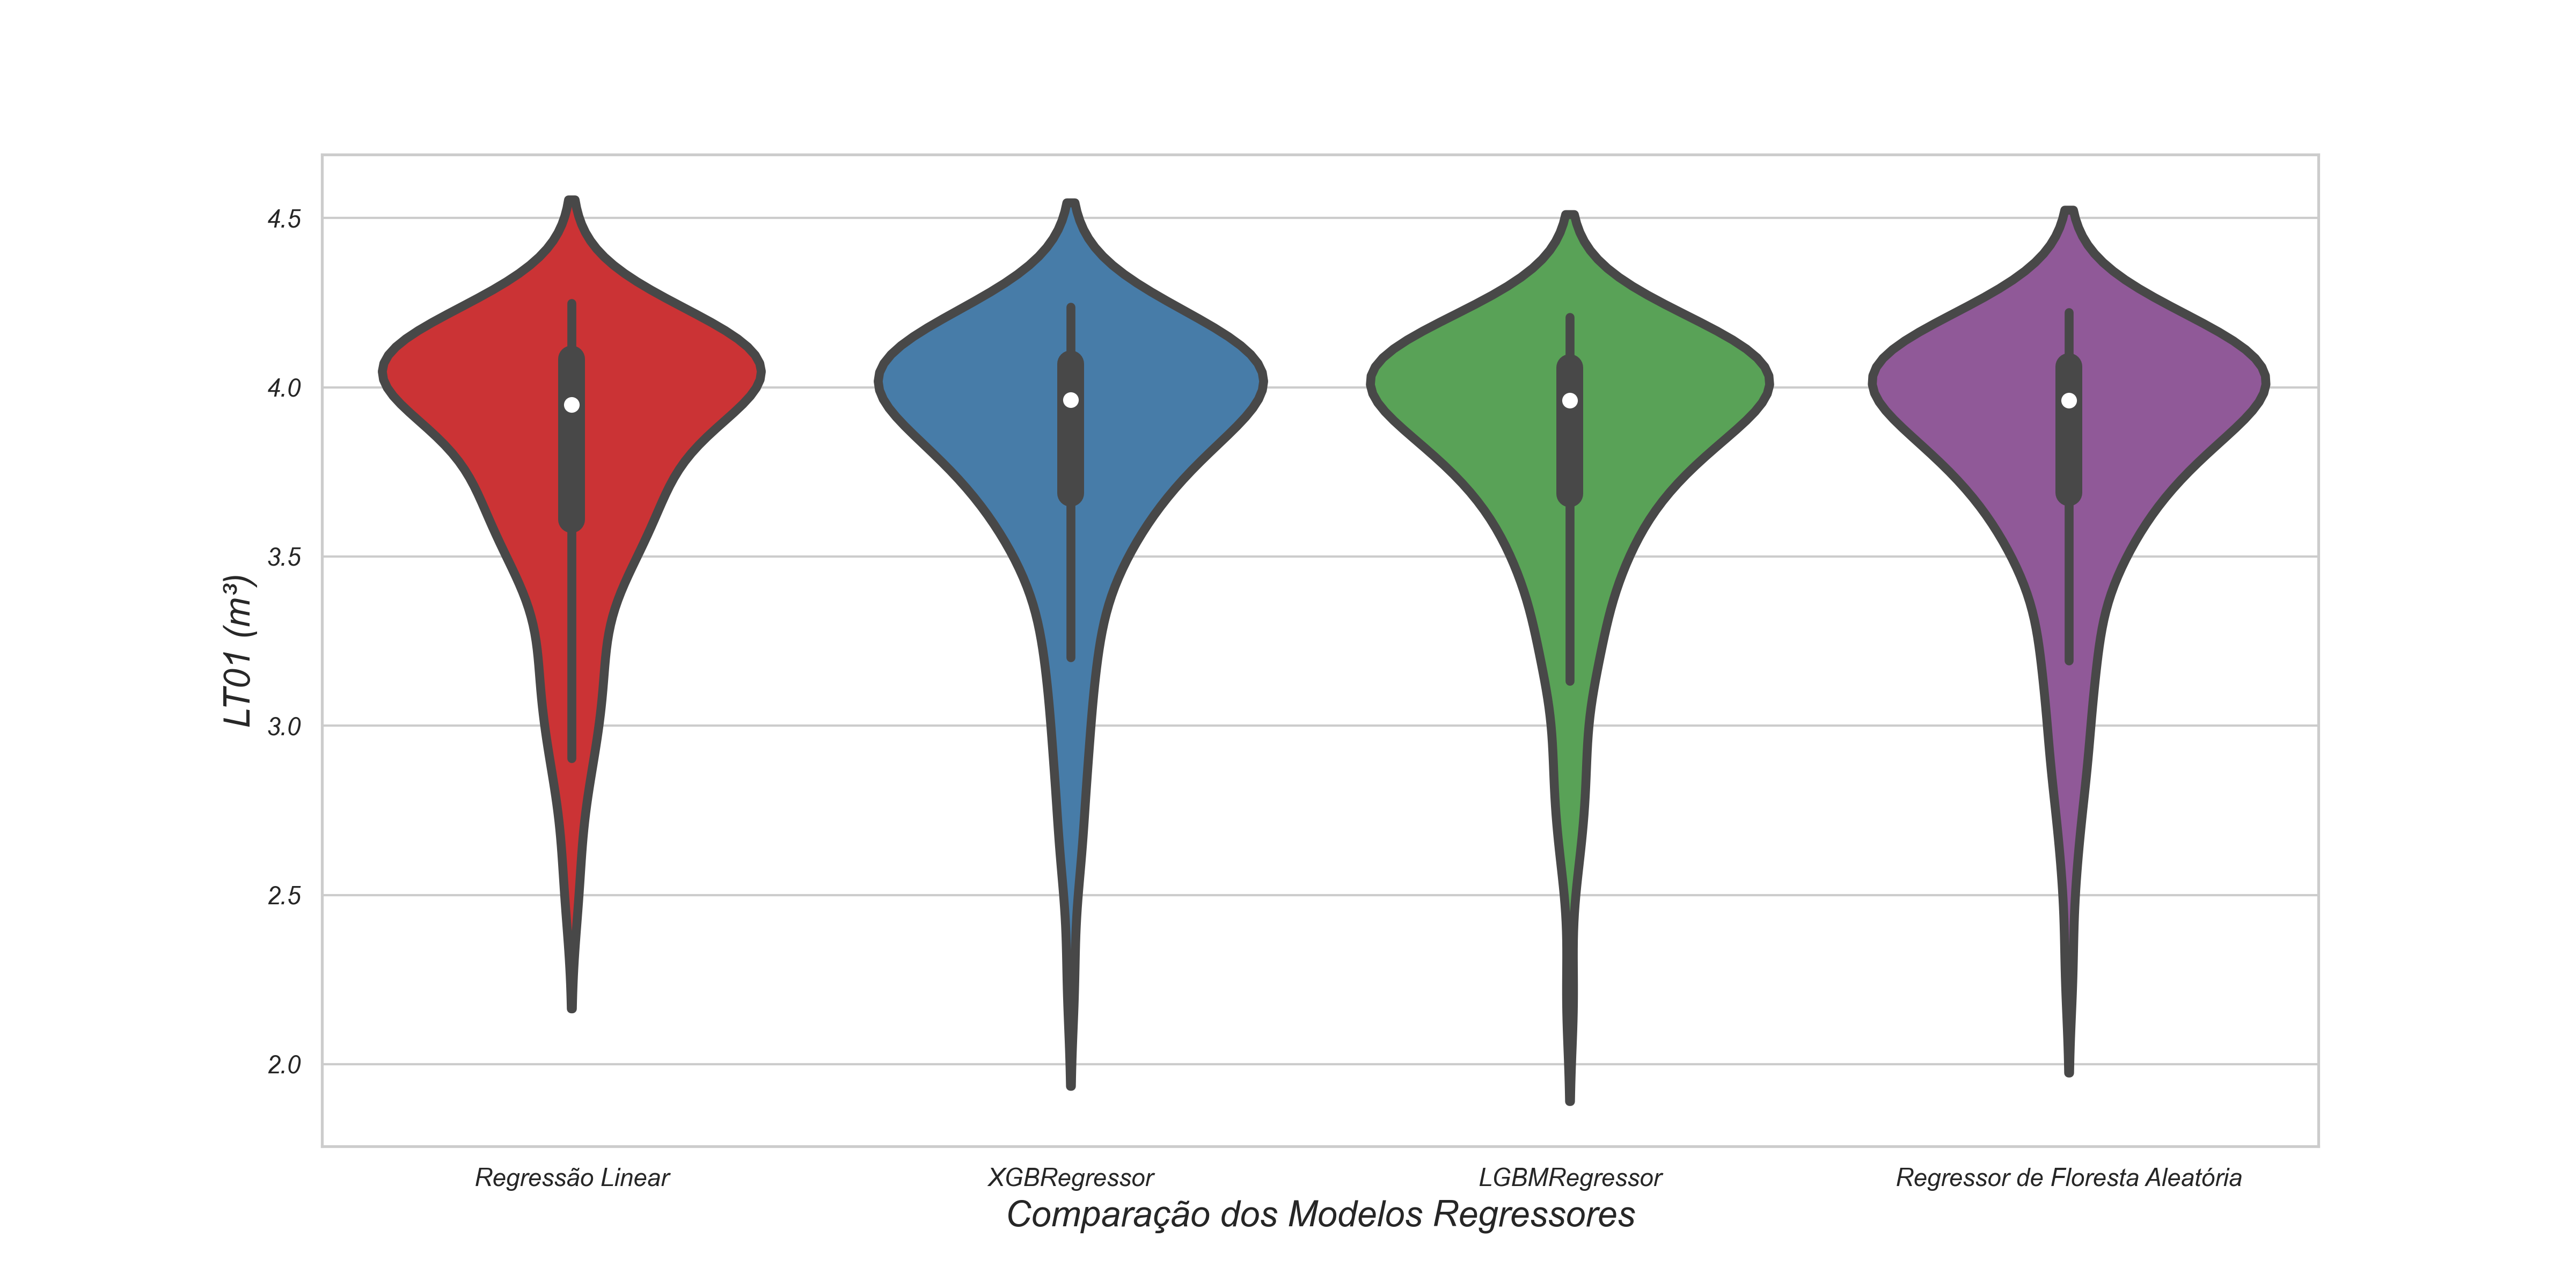
\includegraphics[width=1\linewidth]{Resultados/Figuras/violin-LR-XGB-LGBM-RF}
	
\end{figure}


Na Figura \ref{fig:rrmse_comparar}, nota-se que todos os modelos trabalhados aqui, exceto o modelo LR, foram comparados em relação às métricas de desempenho. Mesmo sendo muito robustos, esses modelos não conseguiram obter um resultado tão bom quanto o RNN.

\begin{figure}[H]
	\centering
	\caption{Análise comparativa dos modelos utilizando gráfico de barras \label{fig:rrmse_comparar} \label{fig:basic_comparar}}
	\begin{subfigure}{1\textwidth}
		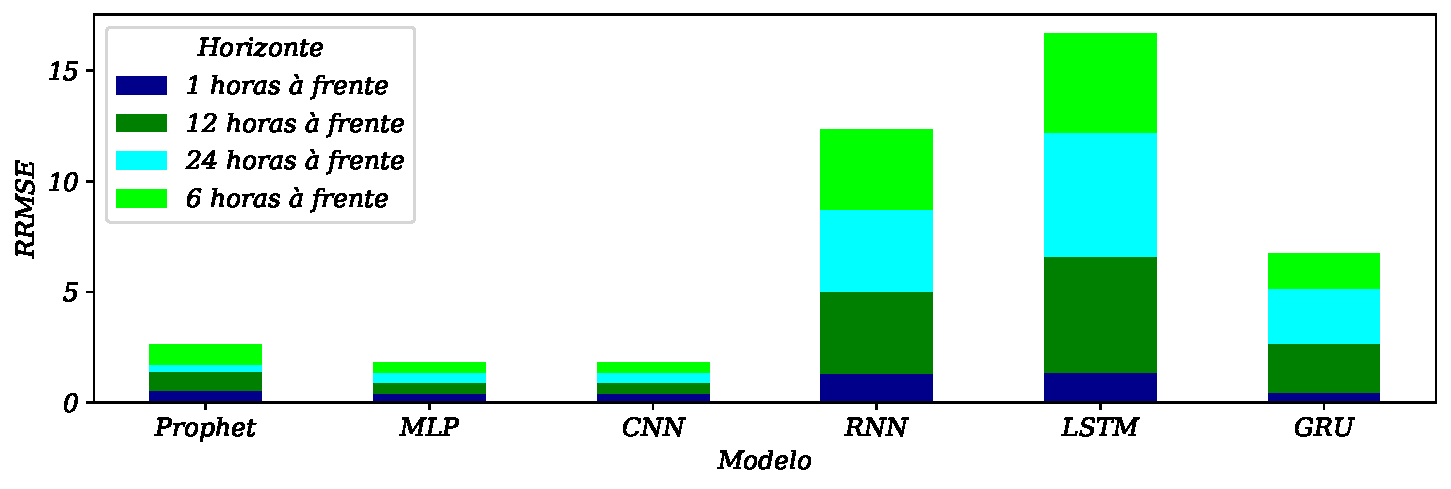
\includegraphics[width=\linewidth]{Resultados/Figuras/rrmse_comparar}
	
		
	\end{subfigure}
	
	\begin{subfigure}{1\textwidth}
		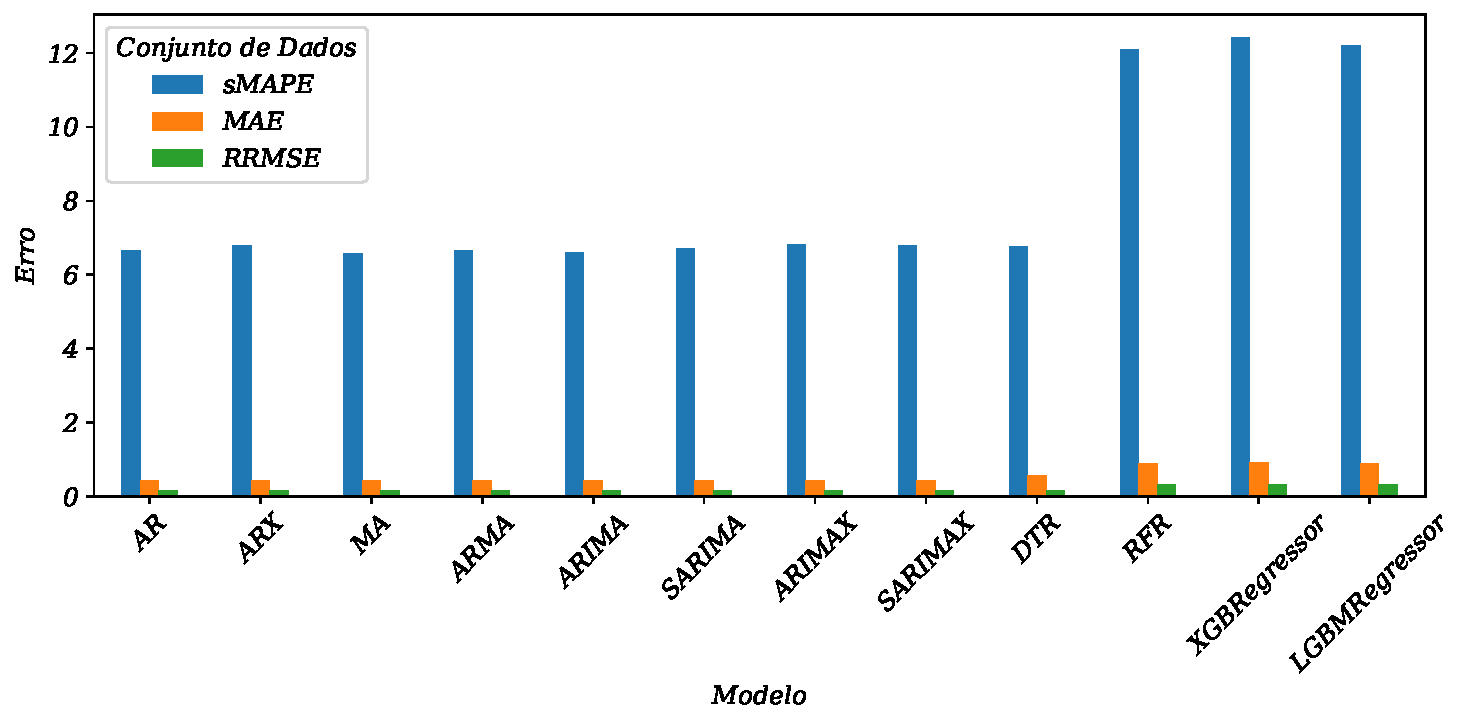
\includegraphics[width=\linewidth]{Resultados/Figuras/basic_comparar}
		
		
	\end{subfigure}
	

\end{figure}

  

\subsection{Aplica\c c\~ao do Mundo Real}\label{subsec:estudo-reslt}


A previsão da demanda de água é uma preocupação fundamental para muitas organizações e autoridades responsáveis pelo abastecimento de água. Neste estudo de caso, explorou-se como a análise de séries temporais pode ser aplicada para prever a demanda de água ao longo do tempo.

A análise de séries temporais é uma abordagem comumente utilizada para prever padrões futuros com base em dados históricos. No estudo, foram aplicadas técnicas de modelagem e previsão, permitindo obter valiosos sobre a demanda de água futura. Diversos modelos, como ARIMA e SARIMA, foram empregados para analisar os dados históricos e gerar previsões confiáveis.
Ao longo do estudo, identificaram-se sazonalidades na demanda de água, bem como padrões de consumo que variam ao longo do tempo. Essas informações são essenciais para o planejamento adequado do abastecimento de água, permitindo uma alocação eficiente dos recursos e uma resposta adequada às flutuações de demanda.

A aplicação da análise de séries temporais na previsão da demanda de água proporciona uma base sólida para a tomada de decisões informadas. Com base nos resultados obtidos, é possível ajustar estratégias de gerenciamento, antecipar picos de demanda e otimizar o uso dos recursos hídricos disponíveis.
Em suma, este estudo demonstrou que a análise de séries temporais é uma abordagem eficaz para prever a demanda de água ao longo do tempo. Ao fornecer precisos e confiáveis, essa técnica contribui para o planejamento e o gerenciamento eficiente do abastecimento de água, promovendo a sustentabilidade e a utilização racional dos recursos hídricos.



\subsubsection{Descri\c c\~ao do Sistema de Abastecimento de \'Agua}



Foram realizadas análises e modelagens utilizando a abordagem de séries temporais para prever a demanda diária de água em uma determinada cidade para os próximos seis meses. Os resultados obtidos forneceram valiosos sobre a demanda futura e contribuíram para um melhor planejamento do abastecimento hídrico. A seguir, apresentam-se as principais conclusões para cada uma das perguntas de pesquisa:

\noindent\ref{q1}: Qual é a adequação da pressão atual para atender à demanda diária?

Após análise dos dados e das métricas utilizadas, conclui-se que a pressão atual é adequada para atender à demanda diária. Durante o período analisado, não foram identificadas situações de pressão insuficiente que afetassem o fornecimento de água.

\noindent\ref{q2}: Qual é o volume mínimo de água necessário no reservatório para evitar o acionamento das bombas durante o horário de pico?

Com base na frequência de funcionamento das bombas e na demanda durante o horário de pico, determinou-se que é necessário manter um volume mínimo de água no reservatório, correspondente a $5285,90$ litros, para evitar o acionamento das bombas nesse período.

\noindent\ref{q3}: Qual é a vazão ótima para atender à demanda diária?

Após análise e modelagem dos dados, identificou-se que a vazão ótima para atender à demanda varia conforme o período do dia e as características sazonais. A pressão necessária para atender à demanda é de $3,60$ PSI (do inglês \textit{pound-force per square inch}) na sucção.

\noindent\ref{q4}: Como encontrar o ponto de equilíbrio entre a demanda e a vazão?

Após análise e modelagem dos dados, foi constatado que não existe um ponto de equilíbrio entre a demanda e a vazão no reservatório. No entanto, identificou-se um volume mínimo de reserva de $3.545$ litros que permite manter um armazenamento adequado no reservatório sem a necessidade de acionar as bombas durante o período de maior custo energético.

Embora essa estimativa de volume mínimo seja importante para garantir o abastecimento contínuo durante o período de pico, é importante ressaltar que não há um equilíbrio perfeito entre a demanda e a vazão nos dados analisados. Portanto, é necessário considerar estratégias adicionais, como otimização do sistema de abastecimento e gerenciamento eficiente dos recursos hídricos, para atender de forma adequada às necessidades da população.

\noindent\ref{q5}: Qual é o impacto do acionamento das bombas durante o horário de pico?

Confirmou-se que a ativação das bombas de sucção durante o período de 18h às 21h resulta em um maior custo energético para a SANEPAR. Portanto, é recomendado evitar o acionamento das bombas durante esse período, utilizando estratégias de armazenamento e gerenciamento eficientes.

\subsubsection{Estudo de Caso 1}\label{subsubsec:quest-est}


As questões de pesquisa levantadas neste estudo foram cuidadosamente abordadas e respondidas ao longo da análise. A seguir, apresenta-se as respostas para cada uma das questões:

\ref{q1} Com base nos resultados obtidos, conclui-se que as pressões atuais das variáveis \textbf{PRESSÃO DE SUCÇÃO - PT01} e \textbf{PRESSÃO DE RECALQUE - PT02} são adequadas para atender à demanda diária. O percentil 10 das pressões de sucção ($3,48$ mca) indica que apenas 10\% dos valores estão abaixo desse limite, o que sugere que a pressão de sucção geralmente se mantém em níveis adequados para o funcionamento adequado do sistema. Da mesma forma, o percentil 90 das pressões de recalque ($24.02$ mca) indica que apenas 10\% dos valores estão acima desse limite, evidenciando que a pressão de recalque também se mantém dentro dos padrões necessários para atender à demanda diária.
Esses resultados indicam que as pressões de sucção e de recalque estão em conformidade com as exigências do sistema, fornecendo a pressão necessária para o adequado abastecimento de água.

\ref{q2} Com base na frequência de funcionamento das bombas e na demanda durante o horário de pico, determinou-se que é necessário manter um volume mínimo de água no reservatório, correspondente a 5285,90 litros, para evitar o acionamento das bombas nesse período.
A vazão ótima para atender à demanda diária do tanque é determinada pelas faixas de fluxo de entrada, gravidade e retorno, juntamente com as faixas de pressão de sucção e retorno. Com base nas informações fornecidas na pergunta \ref{q3}, para manter o tanque quase cheio ou sempre cheio, as seguintes faixas de vazão devem ser consideradas:

Fluxo de entrada: entre $238 \ m^3/h$ e $302 \ m^3/h$;
Fluxo de gravidade: entre $126 \ m^3/h$ e $182 \ m^3/h$;
Fluxo de retorno: entre $110 \ m^3/h$ e $144 \ m^3/h$;
Pressão de sucção: entre $1,92 \ mca$ e $4,24 \ mca$;
Pressão de retorno: entre $21 \ mca$ e $24 \ mca$.
Essas faixas de vazão e pressão garantem que a demanda diária do tanque seja atendida de forma adequada, mantendo o nível de água próximo ao máximo e garantindo a pressão necessária para o funcionamento adequado do sistema de abastecimento de água.


Para responder à pergunta \ref{q4} sobre o ponto de equilíbrio entre a demanda e a vazão, o sistema alcança o equilíbrio quando a vazão da FT01 é de 211 $m^3/h$, a vazão da FT02 é de 114 $m^3/h$, a vazão da FT03 é de 100 $m^3/h$ e o nível do tanque está em 3.545 $m^3$. Nesse ponto de equilíbrio, as bombas não precisam ser acionadas, o que indica que o sistema de abastecimento de água está em uma condição estável. Esses valores de vazão e nível do tanque permitem atender à demanda diária sem a necessidade de tomar medidas adicionais.


\subsubsection{Estudo de Caso 2}

\eqref{q5} Confirmou-se que a ativação das bombas de sucção durante o período de 18h às 21h resulta em um maior custo energético para a SANEPAR. Portanto, é recomendado evitar o acionamento das bombas durante esse período, utilizando estratégias de armazenamento e gerenciamento eficientes.

\eqref{q5}\ref{q5:a} Verificou-se que, para evitar o acionamento das bombas durante o horário de pico (18h às 21h) sem comprometer o abastecimento de água para a população, é necessário manter o nível do reservatório acima de $4.000$ litros.

\eqref{q5}\ref{q5:b} Ao analisar os dados dos últimos 3 anos do Bairro Alto, identificou-se a presença de tendências sazonais e padrões de consumo de água. Essas informações são valiosas para compreender os padrões de demanda e planejar o abastecimento de forma mais eficiente.

\eqref{q5}\ref{q5:c} Observou-se que os horários de pico, nesse caso, correspondem aos períodos em que há maior consumo de água. Esses horários são críticos para o abastecimento, pois a demanda é significativamente maior, exigindo uma gestão cuidadosa dos recursos hídricos nesse intervalo de tempo. É importante monitorar e garantir que haja suprimento adequado nesses horários para atender à demanda da população.



\begin{figure}[H]
	\centering
	\caption{Demanda média das variáveis de fluxo}
	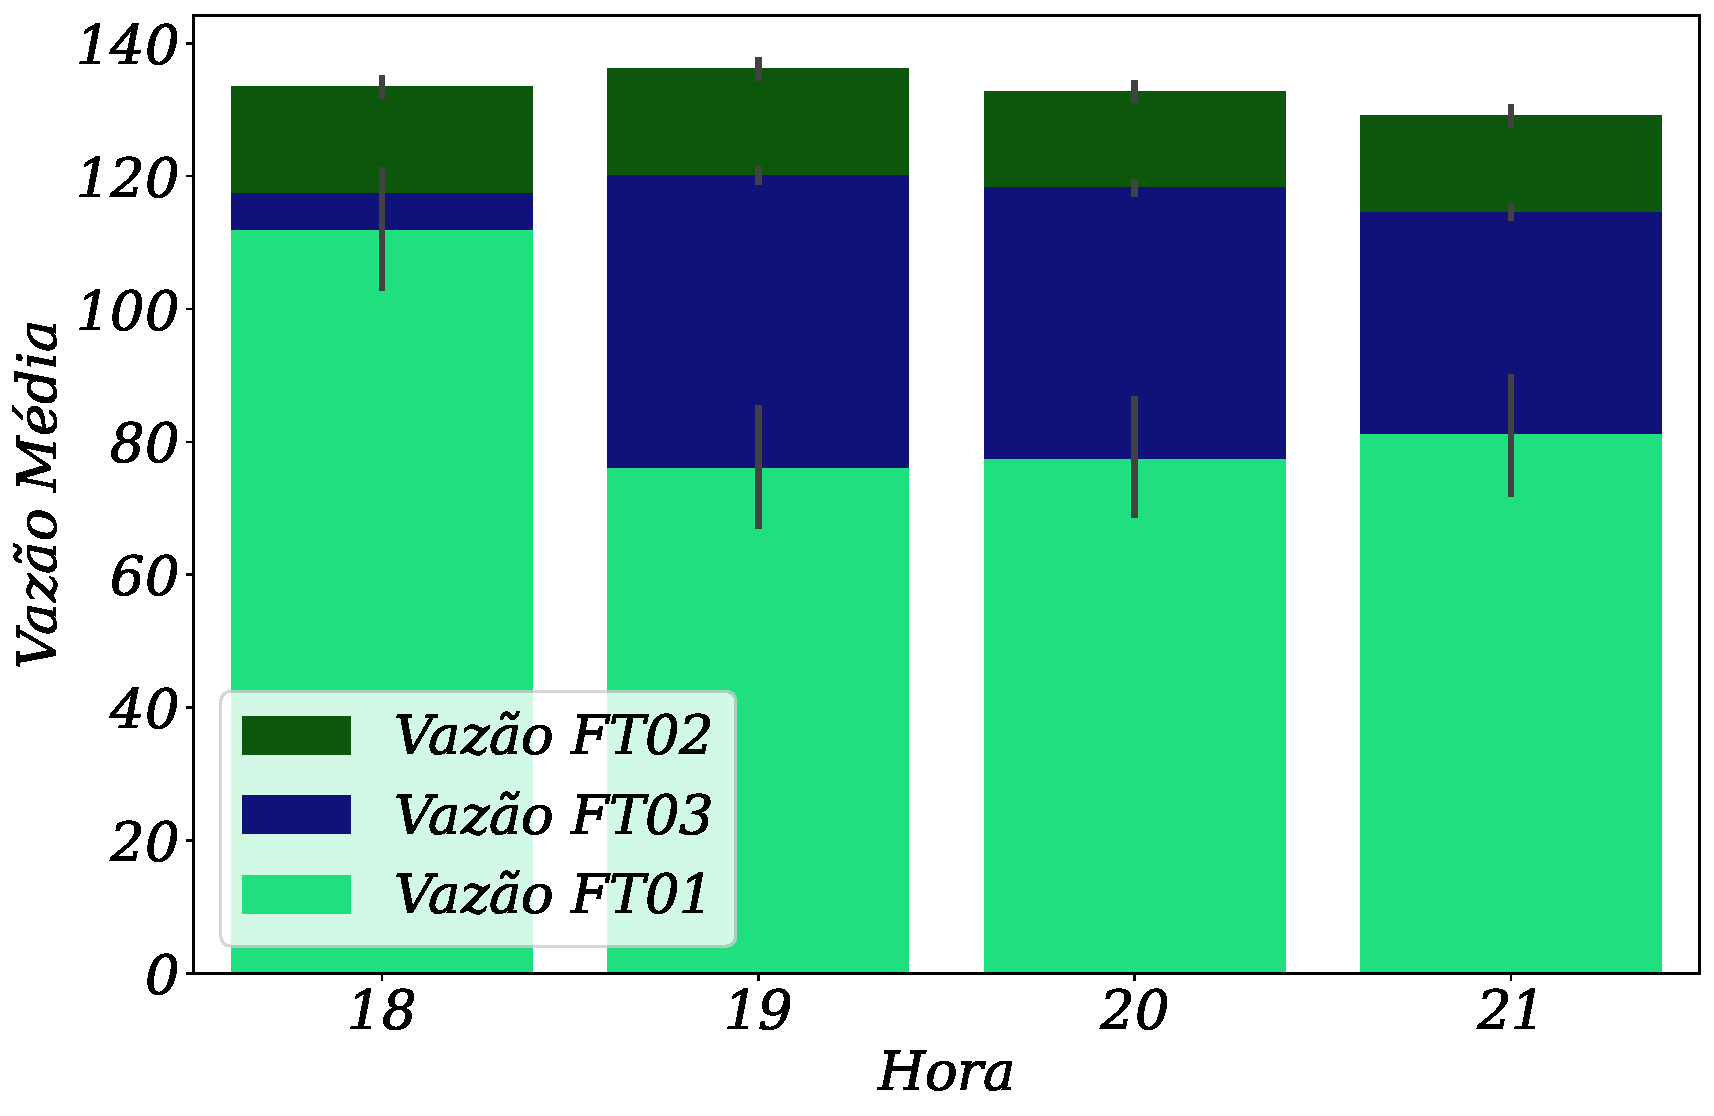
\includegraphics[width=0.9\linewidth]{Resultados/Figuras/grafico-barras-demanda}
	
	\label{fig:grafico-barras-demanda}
	
	\fonte{Elaboração própria a partir de dados da SANEPAR (2018 a 2020)}
\end{figure}

O gráfico de barras apresentado na Figura \ref{fig:grafico-barras-demanda} mostra a demanda média das variáveis de fluxo (Vazão de Entrada-FT01, Vazão de Gravidade-FT02 e Vazão de Recalque-FT03) durante o intervalo das 18h às 21h. Cada barra representa a média da demanda para cada variável em um horário específico dentro desse intervalo. A altura de cada barra indica a magnitude da demanda média para a respectiva variável. Essa visualização permite que sejam identificados os horários em que as variáveis de fluxo apresentaram maior demanda, o que é útil para o planejamento e gerenciamento adequado do sistema.

A questão de pesquisa \ref{q5}\ref{q5:c} foi respondida através da análise dos dados, permitindo a identificação dos horários de maior demanda durante o período das 18h às 21h. A tabela a seguir apresenta os resultados para as três variáveis estudadas: vazão de entrada-FT01, vazão de gravidade-FT02 e vazão de recalque-FT03.




\begin{table}[H]
	\centering
	\caption{Demanda de água}\label{tb:dem}
	\begin{tabular}{@{}ccc@{}}
		\toprule
		\textbf{Variável}         & \textbf{Horário de Maior Demanda} & \textbf{Valor da Demanda} \\ \midrule
		Vazão de entrada - FT01   & 2020/10/08 21:00:00               & $383,87 m^3/h$                   \\
		Vazão de gravidade - FT02 & 2020/10/20 18:00:00               & $326,17 m^3/h$                    \\
		Vazão de recalque - FT03  & 2020/11/26 19:00:00               & $194,35 m^3/h$                    \\ \bottomrule
	\end{tabular}
	
	
	\fonte{Elaboração própria a partir de dados da SANEPAR (2018 a 2020)}
\end{table}

Os resultados destacam os horários específicos em que cada variável apresentou maior demanda dentro do intervalo das 18h às 21h, fornecendo importantes para o planejamento e gerenciamento adequado do sistema. A tabela \ref{tb:dem} resume essas informações.


\eqref{q5}\ref{q5:d} Durante as horas de pico, é necessário que o nível do reservatório esteja mantido dentro na média de $3.9005 \ m^3$ para evitar o acionamento das bombas. Manter o nível do reservatório dentro dessa faixa permitirá que o sistema opere de forma eficiente, atendendo à demanda de água sem a necessidade de acionar as bombas.

\eqref{q5}\ref{q5:e} É importante destacar que a vazão de recalque exerce um impacto mais significativo no nível do reservatório em comparação com as outras vazões. Essa diferença se deve ao fato de que a vazão de recalque está diretamente relacionada à injeção de água no reservatório por meio da bomba localizada próxima à sua base. Em contraste, as demais vazões possuem alguns valores ausentes, o que limita sua influência na análise geral do sistema.







 


